% !TEX program = pdflatex
% !TEX root = ./TP2.tex
%\title{Title page with logo}
%----------------------------------------------------------------------------------------
%	PACKAGES AND OTHER DOCUMENT CONFIGURATIONS
%----------------------------------------------------------------------------------------

\documentclass[12pt]{article}
\usepackage[portuges]{babel}
\usepackage[utf8]{inputenc}
\usepackage[hyphens]{url}
\usepackage{graphicx}
\usepackage[hidelinks]{hyperref}
\usepackage[toc,page]{appendix}
\usepackage{indentfirst}
\usepackage[table,xcdraw]{xcolor}
\usepackage[margin=4cm]{geometry}
\usepackage{pifont}
\usepackage{minted}

\setlength{\parskip}{0.4\baselineskip}%

\newcommand{\tabitem}{~~\llap{\textbullet}~~}
\newcommand{\cmark}{\color[rgb]{0,0.7,0}\ding{51}}%
\newcommand{\xmark}{\color[rgb]{0.7,0,0}\ding{55}}%

\renewcommand\appendixtocname{Anexos}
\renewcommand\appendixpagename{Anexos}

\begin{document}
\sloppy

\begin{titlepage}

\newcommand{\HRule}{\rule{\linewidth}{0.5mm}} % Defines a new command for the horizontal lines, change thickness here

\center % Center everything on the page

\vspace{0.5cm}
 
%----------------------------------------------------------------------------------------
%	HEADING SECTIONS
%----------------------------------------------------------------------------------------

\textsc{\LARGE Scripting no Processamento}\\[0.3cm]
\textsc{\LARGE de Linguagem Natural}\\[1.1cm] % Name of your university/college
\textsc{\Large Universidade do Minho}\\[0.5cm] % Major heading such as course name
\textsc{\large Mestrado Integrado em Engenharia Informática}\\[0.5cm] % Minor heading such as course title

%----------------------------------------------------------------------------------------
%	TITLE SECTION
%----------------------------------------------------------------------------------------
\vspace{0.8cm}
\HRule \\[0.6cm]
{ \huge \bfseries Trabalho Prático 2}\\[0.4cm] % Title of your document
{ \Large \bfseries spaCy's POS Tagging}\\[0.4cm] % Subtitle of your document
\HRule \\[1.0cm]
 
%----------------------------------------------------------------------------------------
%	AUTHOR SECTION
%----------------------------------------------------------------------------------------

\Large \emph{Grupo 7:}\\
A73831 - João Barreira\\
A77364 - Mafalda Nunes\\[1.3cm]

%----------------------------------------------------------------------------------------
%	DATE SECTION
%----------------------------------------------------------------------------------------

{\large \today}\\[1.5cm] % Date, change the \today to a set date if you want to be precise

%----------------------------------------------------------------------------------------
%	LOGO SECTION
%----------------------------------------------------------------------------------------


\includegraphics[width=0.55\textwidth]{logo}\\[1cm] % Include a department/university logo - this will require the graphicx package
 
%----------------------------------------------------------------------------------------

\vfill % Fill the rest of the page with whitespace

\end{titlepage}

\vspace{0.5cm}

\begin{abstract}
O presente relatório tem com objetivo a aprendizagem das funcionalidades da ferramenta \textit{spaCy}. Para tal, apresentar-se-á uma descrição da mesma, mais especificamente da
funcionalidade de POS \textit{tagging}, bem como um pequeno exemplo que demonstre como utilizar a ferramenta.

Este trabalho pretende dar resposta ao trabalho prático 2, proposto na unidade curricular SPLN, do Mestrado em Engenharia Informática, da Universidade do Minho.
\end{abstract}

\vspace{0.5cm}

\tableofcontents

\newpage

\let\oldref\ref
\renewcommand{\ref}[1]{\smash{\underline{\oldref{#1}}}}

\section{spaCy}

O spaCy é uma biblioteca \textit{open-source} para o processamento avançado de linguagem natural em \textit{Python}, que foi desenvolvida especificamente para ser utilizada em ambientes de produção, ajudando a construir aplicações que processam grandes volumes de texto.

Dentro do contexto de processamento de linguagem natural, esta ferramenta pode ser utilizada em muitas vertentes, desde a extração de conhecimento, desenvolvimento de sistemas de compreensão de linguagem natural ou pré-processamento de texto para \textit{deep-learning}.


% Falar sobre o que é
% https://spacy.io/usage/spacy-101
% https://spacy.io/usage/v2

\subsection{Arquitetura} 

As estruturas de dados centrais do spaCy são o \textit{Doc} e o \textit{Vocab}.

\begin{figure}[!ht]
	\centering
	\setlength{\abovecaptionskip}{-.2cm}
	\makebox[\textwidth][c]{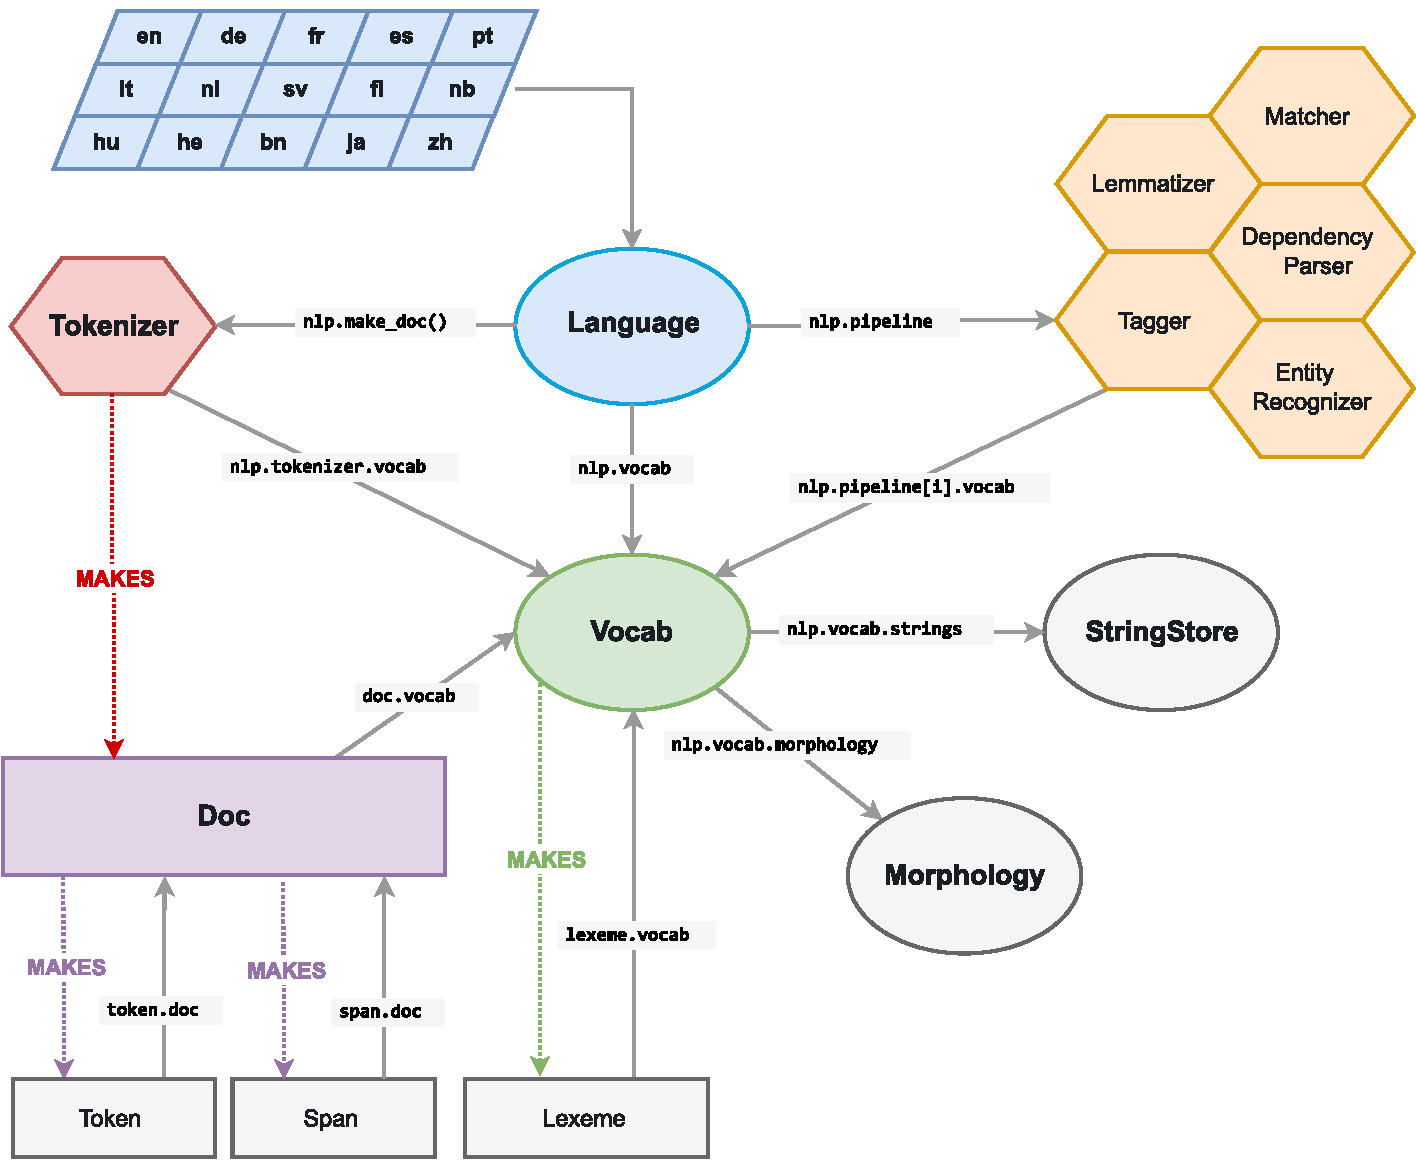
\includegraphics[width=12.8cm]{Pictures/arquitetura}}
	\caption{Esquema da arquitetura do spaCy}
	\label{figure:arquitetura}
\end{figure}

O objeto \textit{Doc} possui uma sequência de \textit{tokens} (palavra, pontuação, espaço em branco, etc.) e de \textit{spans} (porções do objeto \textit{Doc}), bem como todas as respetivas anotações. Os objetos \textit{Span} e \textit{Token} são vistas que apontam para o próprio \textit{Doc}. O \textit{Doc} é construído por um \textit{Tokenizer}, sendo depois modificado pelos componentes de um \textit{Pipeline} (figura \ref{figure:pipelines}). O objeto \textit{Language} coordena estes componentes, ao pegar num texto limpo e enviá-lo para o \textit{pipeline}, retornando um texto anotado. Para além disso, também permite organizar treinamento e serialização de dados.

\begin{figure}[!ht]
	\centering
	\setlength{\abovecaptionskip}{-.8cm}
	\makebox[\textwidth][c]{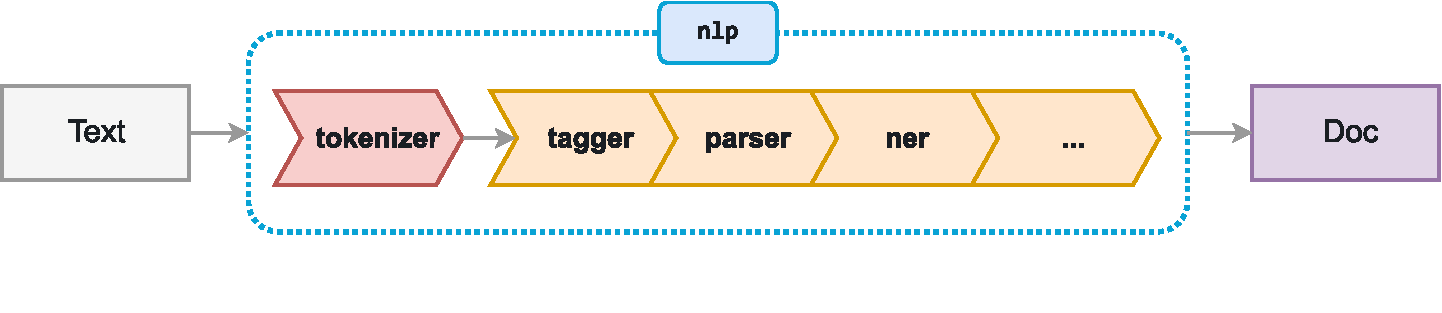
\includegraphics[width=14cm]{Pictures/pipelines}}
	\caption{Esquema representativo da construção do \textit{Doc}}
	\label{figure:pipelines}
\end{figure}

Relativamente aos \textit{pipelines}, é de se destacar os seguintes:
\vspace*{-0.3cm}
\begin{itemize}\itemsep1pt
	\setlength{\itemindent}{+.5cm}	
	\item \texttt{\textit{Lemmatizer}} - permite determinar a forma base de palavras;
	\item \texttt{\textit{Tagger}} - anota \textit{part-of-speech} (POS) \textit{tags} em objetos \textit{Doc};
	\item \texttt{\textit{Matcher}} - faz \textit{match} de sequências de \textit{tokens}, tendo em conta regras padrão, similares a expressões regulares;
	\item \texttt{\textit{DependencyParser}} - anota dependências sintáticas em objetos \textit{Doc};
	\item \texttt{\textit{EntityRecognizer}} - anota nomes de entidades, como pessoas ou produtos, em objetos \textit{Doc}.
\end{itemize}

O objeto \textit{Vocab} possui um conjunto de tabelas de \textit{look-up}, que tornam a informação comum disponível entre documentos. O \textit{Vocab} é constituído por entradas do tipo \textit{Lexeme}, que são um tipo de palavras sem contexto, ao contrário de uma palavra \textit{token}, que possui uma \textit{POS tag}, um parser de dependências, entre outros. O \textit{Vocab} permite também aceder ao objeto \textit{Morphology}, que possibilita a asssociação de características linguísticas, como o \textit{lemma}, o tipo de nome, o tempo verbal, entre outros, aos \textit{tokens}, tendo em conta a palavra e a respetiva \textit{POS tag}. Ao centralizar vetores de palavras, atributos léxicos e \textit{strings}, o spaCy evita armazenar multiplas cópias desses dados, pelo que poupa memória e assegura que existe uma única fonte de verdade. 

Também para poupar memória, o spaCy codifica todas as \textit{strings} para valores de \textit{hash}, que são acessíveis a partir do \textit{StringStore}, que corresponde a um \textit{map} de \textit{strings} de e para valores de \textit{hash}. Internamente, o spaCy apenas trabalha com valores de \textit{hash} (figura \ref{figure:doc-vocab-stringstore}).

\bigskip

\begin{figure}[!ht]
	\centering
	\setlength{\abovecaptionskip}{-.5cm}
	\makebox[\textwidth][c]{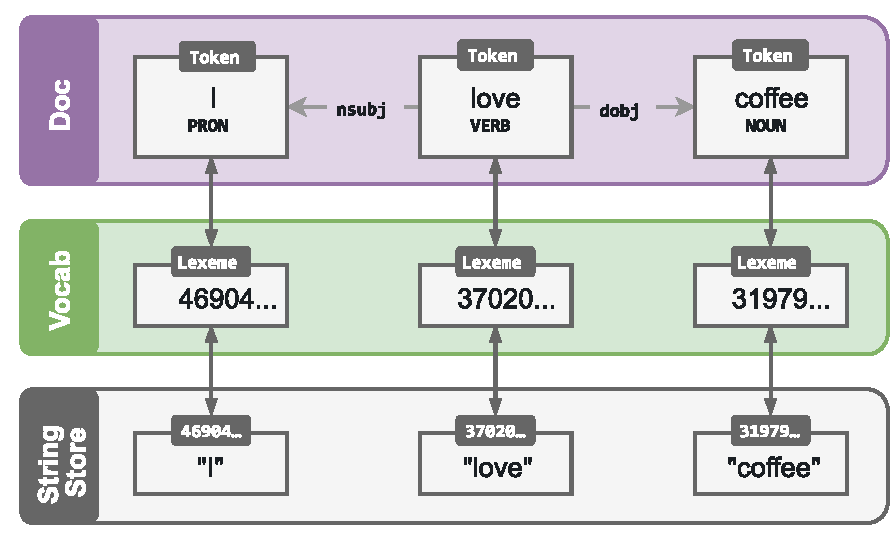
\includegraphics[width=14cm]{Pictures/doc-vocab-stringstore}}
	\caption{Representação esquemática dos objetos \textit{Doc}, \textit{Vocab} e \textit{String Store}}
	\label{figure:doc-vocab-stringstore}
\end{figure}



% https://spacy.io/api/

\subsection{Funcionalidades}

A biblioteca spaCy disponibiliza diversas funcionalidades, sendo que algumas estão associadas a conceitos linguísticos e outras a capacidades mais gerais de \textit{machine learning}. Apesar de algumas destas funcionalidades trabalharem de forma independente, outras requerem o carregamento de modelos estatísticos, para que o spaCy seja capaz de prever anotações linguísticas. Atualmente, o spaCy providencia modelos estatísticos para 8 linguagens, que podem diferir em tamanho, velocidade, utilização de memória, correção e os dados que incluem.

As principais funcionalidades desta biblioteca são sumarizadas de seguida:
\vspace*{-0.3cm}
\begin{itemize}\itemsep1pt
	\setlength{\itemindent}{+.5cm}	
	\item \texttt{\textit{Tokenization}} -- Separação de textos em segmentos significativos, como palavras, pontuação,  entre outros. Esta divisão é efetuada tendo em conta regras específicas de cada linguagem. O \textit{input} corresponde a um texto limpo e o \textit{output} um objeto \textit{Doc}.
	
	\item \texttt{\textit{POS Tagging}} -- atribuir tipos de palavras ou propriedades gramaticais (como verbo ou nome) a \textit{tokens}, que constituem um \textit{Doc}. O spaCy recorre a modelos estatísticos para prever quais as \textit{tags} ou etiquetas que mais provavelmente se aplicam ao contexto currente. As anotações linguísticas do tipo POS são obtidas a partir do atributo \textit{pos\_} do \textit{Token}.
	
	\item \texttt{\textit{Dependency Parsing}} -- Processo de obtenção de relações de dependência entre os elementos de uma frase através de um \textit{parser}. Este \textit{parser} possibilita a iteração do texto \textit{tokenizado} (\textit{Doc}) pelas suas frases nominais, sendo que as dependências são dispostas numa árvore de fácil manipulação. É ainda possível visualizar mais facilmente as dependências de um ou mais \textit{Docs} através de um grafo, cujos arcos possuem uma legenda que caracteriza a ligação sintática entre os \textit{tokens}. 
	
	\item \texttt{\textit{Lemmatization}} -- redução de palavras à sua formas base, sendo frequentemente utilizado para standardizar palavras com significados similares. O \textit{lemma} de 'era' e 'foi', e.g., é 'ser'. Pode-se aceder ao \textit{lemma} através do atributo \textit{lemma\_} do \textit{Token}.
	
	\item \texttt{\textit{Sentence Boundary Detection (SBD)}} -- Processo de separação de frases de um texto separado pelos seus \textit{tokens} (\textit{Doc}). É utilizado o \textit{parsing} de dependências para uma divisão mais correta. Possibilita a definição manual dos limites frásicos (i.e. \textit{boundaries})
	em detrimento dos pré-definidos '.', '!' e '?'.
	
	\item \texttt{\textit{Named Entity Recognition (NER)}} - atribuição de etiquetas ou categorias pré-definidas a nomes correspondentes a objetos do mundo real, como pessoas, companhias, localizações, países, produtos, entre outros. O spaCy reconhece vários tipos de nomes de entidades num documento, através da solicitação de uma previsão ao modelo. Como estes modelos são estatísticos e muito dependentes dos textos com que foram treinados, nem sempre esta previsão é correta, podendo ser necessário posterior processamento específico para o caso em estudo. Os nomes das entidades estão disponíveis na propriedade \textit{ents} de um \textit{Doc} ou na propriedade \textit{ent\_type\_} de um \textit{Token}. Quando se pretende alterar anotações de entidades, tem de se o faze a nível do documento, de forma a assegurar que a sequência de anotações de \textit{tokens} permanece consistente.
	
	\item \texttt{\textit{Similarity}} -- Comparação de dois textos e cálculo de valor que indique quão similares são. A função de similitude compara palavras de um dado texto com base em vetores de palavras específicos para cada linguagem que podem ser customizados para um melhor desempenho em contextos de aplicação específicos.
	
	\item \texttt{\textit{Text Classification}} -- atribuição de categorias ou etiquetas a todo o documento ou partes de um documento.
	
	\item \texttt{\textit{Rule-based matching}} -- Processo de busca de correspondências entre \textit{tokens} e determinados padrões. Estes padrões podem ser bastante complexos, tendo algumas parecenças com o funcionamento expressões regulares. No entanto, podem também tirar partido do conhecimento léxico desta ferramenta, filtrando, por exemplo, por bases morfológicas (i.e. \textit{Lemma}) ou classes gramaticais (i.e. verbos, substantivos, etc.). Possibilita ainda a formulação de padrões mais complexos através de quantificadores, \textit{wildcards}, expressões regulares. Podem ainda ser definidas, de um modo simples, funções que serão chamadas caso se dê uma ou mais correspondências.
	
	\item \texttt{\textit{Training}} -- atualização e melhoria de modelos estatísticos de previsões. Para treinar um modelo, são necessários dados de treino, i.e., exemplos de texto e etiquetas (POS \textit{tag}, \textit{named entity}, etc.) que se pretende que o modelo seja capaz de prever. O modelo pode ser melhorado através do processamento de novos textos limpos, em que o utilizador, que conhece a correção da resposta, dá \textit{feedback} ao modelo sobre a sua previsão na forma de um gradiente de erro da função de perda que calculam a diferença entre o exemplo de treino e o \textit{output} esperado (figura \ref{figure:training}). Quanto maior a diferença, mais significativo o gradiente e as atualizações ao modelo.

	\item \texttt{\textit{Serialization}} -- Funcionalidade responsável por guardar objetos do \textit{spaCy} para ficheiros em disco, bem como por carregar objetos previamente guardados. Este processo torna-se especialmente importante quando usado para guardar objetos do tipo \textit{Doc}, por exemplo, que possuem todas as informações retiradas do texto original, bem como outras características inseridas manualmente como entidades ou vetores de palavras customizados. Para isso, é utilizado  a biblioteca \textit{Pickle}, \textit{built-in} da linguagem \textit{Python}.
\end{itemize}



\begin{figure}[!ht]
	\centering
	\setlength{\abovecaptionskip}{-.4cm}
	\makebox[\textwidth][c]{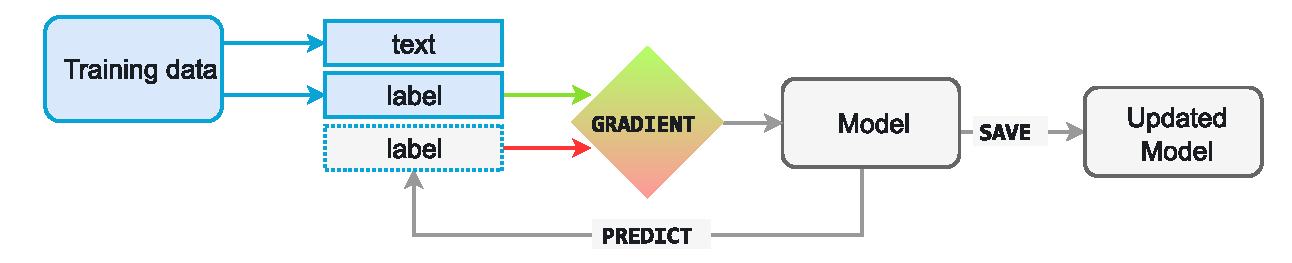
\includegraphics[width=14cm]{Pictures/training}}
	\caption{Esquema representativo do funcionamento do processo de treino}
	\label{figure:training}
\end{figure}

% fala um bocadinho mais de reconhecimento de entidades e grafos de dependencias

% https://spacy.io/usage/spacy-101
% https://spacy.io/usage/linguistic-features
%% https://spacy.io/usage/processing-pipelines
%% https://spacy.io/usage/vectors-similarity
% https://spacy.io/usage/training
%% https://spacy.io/usage/adding-languages
%% https://spacy.io/usage/visualizers

%% https://spacy.io/usage/v2
%% https://spacy.io/api/annotation
%% https://spacy.io/api/top-level

% https://towardsdatascience.com/a-short-introduction-to-nlp-in-python-with-spacy-d0aa819af3ad
%%https://towardsdatascience.com/a-review-of-named-entity-recognition-ner-using-automatic-summarization-of-resumes-5248a75de175


\subsection{Vantagens} % Mafalda

Existem diversas ferramentas do género do spaCy que podem ser utilizadas para efetuar processamento de linguagem natural. Assim, há que apresentar as principais distinções entre estas, de forma a perceber qual será a que trará mais vantagens na sua utilização.

Em primeiro lugar, pode-se efetuar uma breve comparação entre as funcionalidades oferecidas pelo spaCy e outras ferramentas semelhantes, como SyntaxNet, NLTK e CoreNLP.

\begin{table}[!ht]
	\centering
	\renewcommand{\arraystretch}{1.3}
	\begin{tabular}{l|c|c|c|c|}
		\cline{2-5}
	& \cellcolor[HTML]{C0C0C0}\textbf{spaCy} & \cellcolor[HTML]{C0C0C0}\textbf{SyntaxNet} & \cellcolor[HTML]{C0C0C0}\textbf{NLTK} & \cellcolor[HTML]{C0C0C0}\textbf{CoreNLP} \\ \hline
	\multicolumn{1}{|l|}{\cellcolor[HTML]{C0C0C0}Programming language}
	& Python   & C++      & Python   & Java     \\ \hline
	\multicolumn{1}{|l|}{\cellcolor[HTML]{C0C0C0}Neural network models}
	&  \cmark  &  \cmark  &  \xmark  &  \cmark  \\ \hline
	\multicolumn{1}{|l|}{\cellcolor[HTML]{C0C0C0}Integrated word vectors}
	&  \cmark  &  \xmark  &  \xmark  &  \xmark  \\ \hline
	\multicolumn{1}{|l|}{\cellcolor[HTML]{C0C0C0}Multi-language support}
	&  \cmark  &  \cmark  &  \cmark  &  \cmark  \\ \hline
	\multicolumn{1}{|l|}{\cellcolor[HTML]{C0C0C0}Tokenization}
	&  \cmark  &  \cmark  &  \cmark  &  \cmark  \\ \hline
	\multicolumn{1}{|l|}{\cellcolor[HTML]{C0C0C0}Part-of-speech tagging}
	&  \cmark  &  \cmark  &  \cmark  &  \cmark  \\ \hline
	\multicolumn{1}{|l|}{\cellcolor[HTML]{C0C0C0}Sentence segmentation}
	&  \cmark  &  \cmark  &  \cmark  &  \cmark  \\ \hline
	\multicolumn{1}{|l|}{\cellcolor[HTML]{C0C0C0}Dependency parsing}
	&  \cmark  &  \cmark  &  \xmark  &  \cmark  \\ \hline
	\multicolumn{1}{|l|}{\cellcolor[HTML]{C0C0C0}Entity recognition}
	&  \cmark  &  \xmark  &  \cmark  &  \cmark  \\ \hline
	\multicolumn{1}{|l|}{\cellcolor[HTML]{C0C0C0}Coreference resolution}
	&  \xmark  &  \xmark  &  \xmark  &  \cmark  \\ \hline
	\end{tabular}
	\caption{Funcionalidades de diversas ferramentas NLP}
	\label{table:campare_features}
\end{table}

Como se pode perceber através da análise da tabela \ref{table:campare_features}, o spaCy disponibiliza todas as principais funcionalidades associadas o processamento de linguagem natural, exceto a \textit{Conference Resolution}, que corresponde à tarefa de encontrar todas as expressões que se referem à mesma entidade num texto. Apenas o CoreNLP possui essa capacidade, sendo que, em contrapartida, não possui \textit{Integrated word vectors}, que possibilitam a previsão de quão similares são dois objetos. Assim, percebe-se que o spaCy será a melhor alternativa em muitos dos casos.

Outro fator fundamental na comparação entre o spaCy e outras ferramentas semelhantes, é o desempenho, i.e., o tempo que o spaCy demora a gerar respostas. Dois artigos revistos em 2015 ({{REF}}) confirmam que o spaCy oferece o \textit{parser} sintático mais rápido do mundo e que a sua precisão está dentro de 1\% do melhor disponível. Os poucos sistemas mais precisos são pelo menos 20 vezes mais lentos. Alguns valores de precisão e velocidade são apresentados na tabela \ref{table:campare_benchmarks}. Informações mais detalhadas relativamente à velocidade são apresentadas na tabela \ref{table:campare_speed}.

\begin{table}[!ht]
	\centering
	\renewcommand{\arraystretch}{1.3}
	\begin{tabular}{|
		>{\columncolor[HTML]{C0C0C0}}l |c|c|c|c|}
		\hline
		\multicolumn{1}{|c|}{\cellcolor[HTML]{C0C0C0}\textbf{System}} & \cellcolor[HTML]{C0C0C0}\textbf{Year} & \cellcolor[HTML]{C0C0C0}\textbf{Language} & \cellcolor[HTML]{C0C0C0}\textbf{Accuracy} & \cellcolor[HTML]{C0C0C0}\textbf{Speed (wps)} \\ \hline
		spaCy v2.x  & 2017   & Python/Cython  & 92.6       & n/a       \\ \hline
	spaCy v1.x  & 2015   & Python/Cython  & 91.8       & 13,963    \\ \hline
	ClearNLP    & 2015   & Java           & 91.7       & 10,271    \\ \hline
	CoreNLP     & 2015   & Java           & 89.6       & 8,602     \\ \hline
	MATE        & 2015   & Java           & 92.5       & 550       \\ \hline
	Turbo       & 2015   & C++            & 92.4       & 349       \\ \hline
	\end{tabular}
	\caption{Precisão e velocidade de várias ferramentas NLP}
	\label{table:campare_benchmarks}
\end{table}

\begin{table}[!ht]
	\centering
	\renewcommand{\arraystretch}{1.3}
	\begin{tabular}{l|c|c|c|c|c|c|}
	\cline{2-7}
	& \multicolumn{3}{c|}{\cellcolor[HTML]{C0C0C0}\textbf{Absolute (ms per doc)}} & \multicolumn{3}{c|}{\cellcolor[HTML]{C0C0C0}\textbf{Relative (to spaCy)}} \\ \hline
	\rowcolor[HTML]{C0C0C0} 
	\multicolumn{1}{|c|}{\cellcolor[HTML]{C0C0C0}\textbf{System}} & \textbf{Tokenize}      & \textbf{Tag}      & \textbf{Parse}     & \textbf{Tokenize}     & \textbf{Tag}     & \textbf{Parse}     \\ \hline
	\multicolumn{1}{|l|}{\cellcolor[HTML]{C0C0C0}spaCy}
	& 0.2ms   & 1ms    & 19ms    & 1x     & 1x    & 1x     \\ \hline
	\multicolumn{1}{|l|}{\cellcolor[HTML]{C0C0C0}CoreNLP}
	& 0.18ms  & 10ms   & 49ms    & 0.9x   & 10x   & 2.6x   \\ \hline
	\multicolumn{1}{|l|}{\cellcolor[HTML]{C0C0C0}ZPar}
	& 1ms     & 8ms    & 850ms   & 5x     & 8x    & 44.7x  \\ \hline
	\multicolumn{1}{|l|}{\cellcolor[HTML]{C0C0C0}NLTK}
	& 4ms     & 443ms  & n/a     & 20x    & 443x  & n/a    \\ \hline
	\end{tabular}
	\caption{Informações detalhadas sobre velocidade de diversas ferramentas NLP}
	\label{table:campare_speed}
\end{table}

A partir das informações das tabelas \ref{table:campare_benchmarks} e \ref{table:campare_speed}, percebe-se que o spaCy deverá ser uma boa escolha, também em termos de precisão e desempenho.

Há, contudo, que se ter em atenção o tipo de texto que se irá utilizar e o tipo de processamento que se pretende efetuar, uma vez que os valores de precisão, o tamanho do modelo e a velocidade de processamento dependem de vários fatores, como, por exemplo, a linguagem ou modelo utilizado.

% Artigos:
% https://aclweb.org/anthology/P/P15/P15-1038.pdf
% https://www.aclweb.org/anthology/D/D15/D15-1162.pdf


% https://spacy.io/usage/facts-figures


%% Este apresenta o recall, mas tem menos exemplos... 
%%https://www.analyticsvidhya.com/blog/2017/04/natural-language-processing-made-easy-using-spacy-%E2%80%8Bin-python/

%% https://medium.com/@brianray_7981/ai-in-practice-identifying-parts-of-speech-in-python-8a690c7a1a08

\subsection{Utilização} % João

O processo de instalação da biblioteca é bastante simples, podendo ser realizado através do \textit{pip} (\textit{package manager} da linguagem \textit{Python}), utilizado, neste
exemplo, na sua versão 3.X.

\begin{verbatim}
	$ pip3 install spacy
\end{verbatim}

Os modelos correspondentes às linguagens podem ser também facilmente obtidos através do seguinte comando abaixo, exemplificado para um dos modelos da língua inglesa.

\begin{verbatim}
	$ python3 -m spacy download en_core_web_sm
\end{verbatim}

Após o processo de instalação da biblioteca e de \textit{download} das linguagens, o primeiro passo será importar a biblioteca. Depois, poder-se-á carregar a linguagem já
descarregada e produzir um \textit{Doc} a partir de um qualquer texto. Será então possível começar imediatamente a tirar proveito das funcionalidades providenciadas pela biblioteca,
utilizando o objeto do tipo \textit{Doc} resultante do processamento do texto inserido.

\begin{verbatim}
	>>> import spacy
	>>> nlp = spacy.load('en_core_web_sm')
	>>> doc = nlp('This text can now be processed using spaCy!')
\end{verbatim}

% https://spacy.io/api/cli
% https://spacy.io/usage/

\subsection{Aplicações}

Com todas as funcionalidades do spaCy, consegue-se concretizar diversos tipos de processamento de texto de forma geralmente simples. Algumas possibilidades são as que se indicam de seguida:
\vspace*{-0.3cm}
\begin{itemize}\itemsep1pt
	\setlength{\itemindent}{+.5cm}	
	\item desenhar os gráficos de dependências num texto;
	\item reconhecer entidades num texto;
	\item extrair relações entre frases e entidades utilizando as funcionalidades de \textit{entity recognizer} e de \textit{dependency parse};
	\item obter marcações de um conjunto personalizado de entidades, alterando-se para isso anotações de entidades com base, e.g., numa lista de nomes desse conjunto e juntando-se entidades num único \textit{token};
	\item corrigir ou personalizar atributos nos objetos \textit{Doc}, \textit{Span} e/ou \textit{Token};
	\item treinar o \textit{Named Entity Recognizer}, o \textit{Dependency Parser}, o \textit{Part-of-speech Tagger} ou o \textit{Text Classifier} do spaCy, partindo de um modelo já treinado ou de um em branco;
\end{itemize}

% https://spacy.io/usage/examples
% https://github.com/explosion/spacy/blob/master/examples/information_extraction/entity_relations.py

Estes exemplos apresentados são de implementação relativamente fácil, tendo-se concretizado alguns dos mais simples.

\subsubsection{Grafos de Dependências}

Relativamente ao desenho dos grafos de dependências, é possível desenvolver uma função que os imprima para ficheiros com formato \textit{svg} ou para \textit{html}, sendo esta apresentada no excerto de código do anexo \ref{anexo:working_example_1}) com o nome de \textit{generate\_dependencies\_graph}.

Para obter as dependências dentro de cada frase, basta separar as mesmas do objeto \textit{Doc} e invocar sobre estas a função \textit{serve} (mostra no \textit{browser}) ou \textit{render} (devolve conteúdo a guardar num documento \textit{svg} ou \textit{html}) com o estilo \textit{dep}. Existem outras formas de realizar esta tarefa, mas esta é a mais simples e ainda permite personalizar o grafo gerado, como mudar a cor do fundo, tipo de letra, entre outros.

Esta função pode ser utilizada da seguinte forma:

\begin{verbatim}
	>>> import spacy
	>>> from spacy import displacy
	>>> nlp = spacy.load('pt')
	>>> doc = nlp('Pretende-se gerar o gráfico de dependências do
	spaCy!')
	>>> generate_dependencies_graph(doc)

		Serving on port 5000...
		Using the 'dep' visualizer
	
\end{verbatim}

Acedendo-se ao endereço \texttt{127.0.0.1:5000/} no \textit{browser}, obtém-se o resultado apresentado na figura \ref{figure:dependencies-graph}. Também se poderia solicitar o output em ficheiro(s) \textit{html} ou \textit{svg}, aterando o argumento \textit{type}. Nesse caso, o conteúdo dos ficheiros seria retornado pela função. Os restantes argumentos, também opcionais, conferem diferentes características estéticas ao \textit{output}.

\begin{figure}[!ht]
	\centering
	\setlength{\abovecaptionskip}{-.5cm}
	\makebox[\textwidth][c]{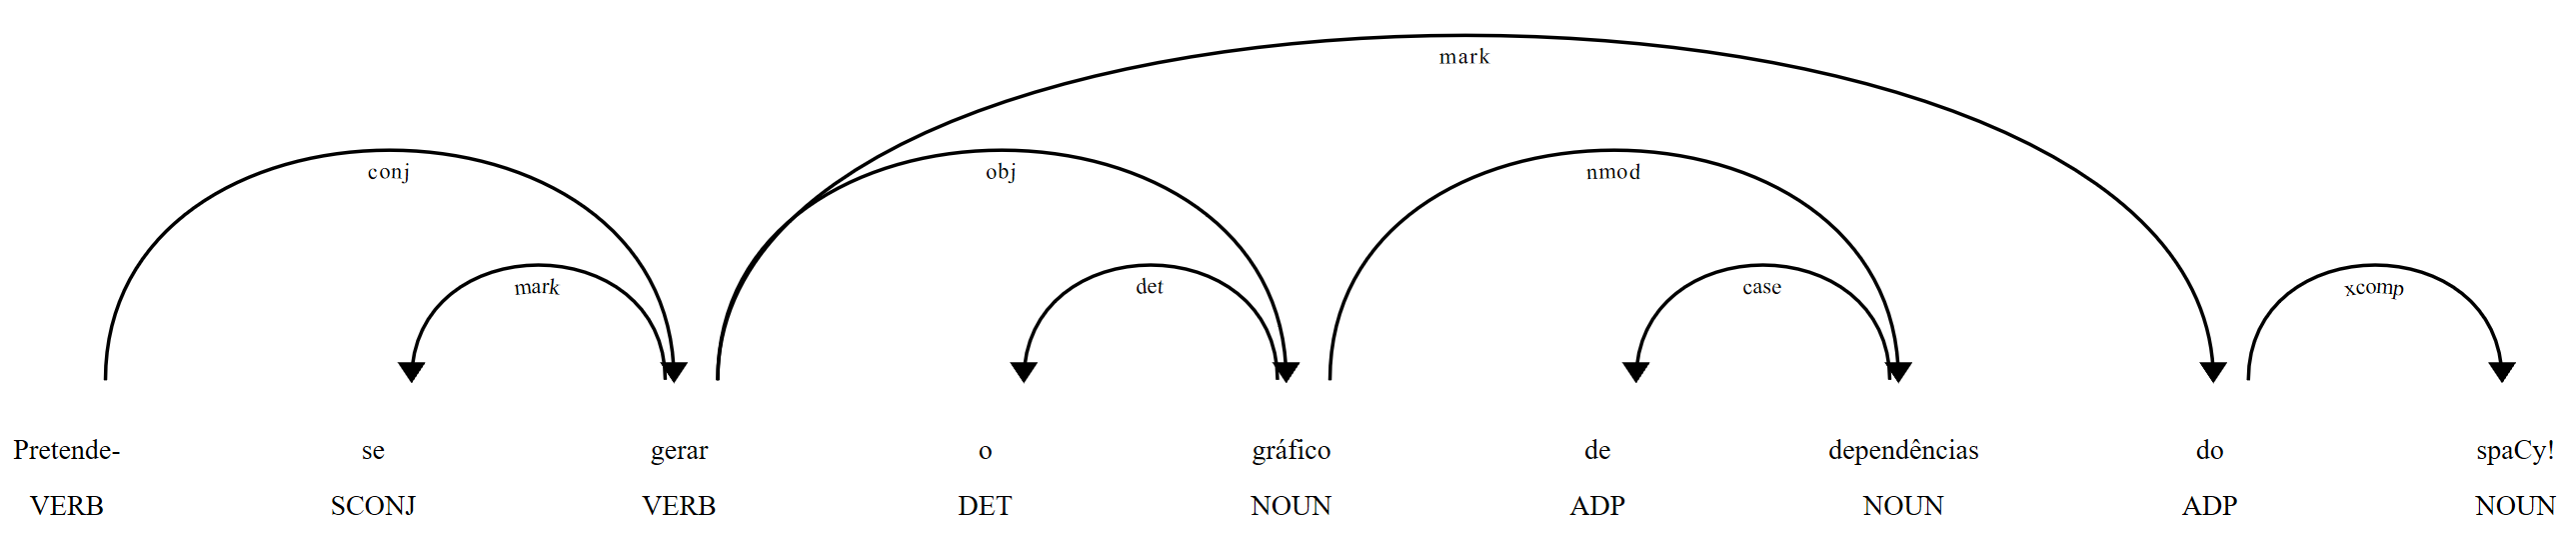
\includegraphics[width=14cm]{Pictures/dependencies_graph}}
	\caption{\textit{Output} de invocação da função \textit{generate\_dependencies\_graph}}
	\label{figure:dependencies-graph}
\end{figure}


\subsubsection{Reconhecimento de Entidades}

Para se proceder ao reconhecimento de entidades, desenvolveu-se a função \textit{generate\_tagged\_text} do excerto de código do anexo \ref{anexo:working_example_1}). Essa função permite obter resultados no \textit{browser}, em ficheiros \textit{html} ou na \textit{shell}. 

Para desenvolver esta funcionalidade, basta invocar sobre o \textit{Doc} a função \textit{displacy.serve} (mostra no \textit{browser}) ou \textit{displacy.render} (devolve conteúdo a guardar num documento \textit{html}) com o estilo \textit{ent}. Para se obter o \textit{output} em formato de texto, percorreu-se todos os \textit{tokens} do \textit{Doc} e, caso este tivesse uma entidade associada (atributo \textit{ent\_typ\_}), a mesma seria escrita junto ao \textit{token}.

Esta função pode ser utilizada da seguinte forma, para obter o \textit{output} no \textit{browser}:

\begin{verbatim}
	>>> import spacy
	>>> from spacy import displacy
	>>> nlp = spacy.load('pt')
	>>> doc = nlp('Hoje o Manuel gostava de ir ao cinema do Braga
	Parque!')
	>>> generate_tagged_text(doc)

		Serving on port 5000...
		Using the 'ent' visualizer
	
\end{verbatim}

Acedendo-se ao endereço \texttt{127.0.0.1:5000/} no \textit{browser}, obtém-se o resultado apresentado na figura \ref{figure:ent-tagger}. Também se poderia solicitar o output em ficheiro \textit{html}, aterando o argumento \textit{type}. Nesse caso, o conteúdo do ficheiro seria retornado pela função. O atributo \textit{entities} permite indicar quais as entidades que se pretendem etiquetar. Caso nenhuma seja indicada, todas são etiquetadas. O argumento \textit{color}, também opciona, confere diferentes cores aos \textit{labels} das entidades.


\begin{figure}[!ht]
	\centering
	\setlength{\abovecaptionskip}{-.5cm}
	\makebox[\textwidth][c]{
\includegraphics[width=14cm]{Pictures/ent_tagger}}
	\caption{\textit{Output} de invocação da função \textit{generate\_tagged\_text}}
	\label{figure:ent-tagger}
\end{figure}

Caso se pretenda obter o resultado em texto, pode-se realizar o seguinte comando:

\begin{verbatim}
	>>> generate_tagged_text(doc, 'text')
	
	'Hoje o Manuel{PER} gostava de ir a o cinema do Braga{ORG}
	Parque{ORG} !'

\end{verbatim}


\subsubsection{Especificação de \textit{Tokens}}

Com o spaCy consegue-se, de forma bastante simples, alterar informação associada a determinado \textit{Token}, ou gerar uma nova divisão para determinada palavra. A palavra inglesa \textit{don't}, e.g., é geralmente dividida em \textit{do} e \textit{n't} (\textit{not}), mas tal não se verifica no Reino Unido, onde esta deve permanecer sempre um único \textit{Token}.

A função \textit{add\_tokenizer\_exceptions}, apresentada no excerto de código do anexo \ref{anexo:working_example_1}, demonstra como personalizar um \textit{Token}, ao adicionar ao \textit{Tokenizer} do modelo casos especiais.O argumento \textit{tokens} dessa função deverá ser um dicionário, em que a chave é o \textit{Token} original e o valor é uma lista de dicionários. Esta lista de dicionários corresponde aos atributos do \textit{Token}, devendo conter o nome do atributo e o respetivo valor como chave e valor, respetivamente. Note-se que o atributo \textit{ORTH} deve ser sempre especificado e, todos concatenados, devem formar o \textit{Token} original.


A referida função pode ser utilizada da seguinte forma:

\begin{verbatim}
	>>> import spacy
	>>> nlp = spacy.load('en_core_web_lg')
	>>> doc = nlp("We don't need to go now!")
	>>> [print((token.orth_, token.lemma_, token.tag_, 
	token.pos_)) for token in doc]
	('We', '-PRON-', 'PRP', 'PRON')
	('do', 'do', 'VBP', 'VERB')
	("n't", 'not', 'RB', 'ADV')
	('need', 'need', 'VB', 'VERB')
	('to', 'to', 'TO', 'PART')
	('go', 'go', 'VB', 'VERB')
	('now', 'now', 'RB', 'ADV')
	('!', '!', '.', 'PUNCT')

	>>> tokens = {"don't": [{'ORTH': 'do', 'LEMMA': 'do',
	'POS': 'VERB'}, {'ORTH': "n't", 'LEMMA': 'not'}]}
	>>> doc = nlp("We don't need to go now!")
	>>> [print((token.orth_, token.lemma_, token.tag_,
	token.pos_)) for token in doc]
	('We', '-PRON-', 'PRP', 'PRON')
	("don't", "don't", '', 'VERB')
	('need', 'need', 'VB', 'VERB')
	('to', 'to', 'TO', 'PART')
	('go', 'go', 'VB', 'VERB')
	('now', 'now', 'RB', 'ADV')
	('!', '!', '.', 'PUNCT')
\end{verbatim}


\subsubsection{Treino do \textit{dependency parser}}

Como foi dito anteriormente, o \textit{spaCy} possibilita o treino de novos modelos estatísticos utilizados nas suas mais diversas funcionalidades. Umas dessas funcionalidades, demonstrada neste exemplo, é o \textit{dependency parser}.

Em primeiro lugar, é criada uma variável \textit{TRAIN\_DATA} que possui duas frases nominais, bem como o nome das dependências (\textit{deps}) e quais os elementos principais dessas mesmas dependências (\textit{heads}). Esta variável servirá como base para o processo de treino. De seguida, é criada a linguagem que poderá ser uma das pré-existentes, ou criada de raíz (i.e. \textit{blank}). Depois, é adicionado o \textit{parser} à \textit{pipeline} e adicionadas as etiquetas com os nomes das dependências ao \textit{parser} que é finalmente utilizado para treinar a linguagem utilizando a variável \textit{TRAIN\_DATA} criada anteriormente. O resultado é, a seguir, testado, através da impressão do resultado das dependências para um novo texto.

Adicionalmente, tira-se ainda partido da capacidade de serialização do \textit{spaCy} (abordada anteriormente neste relatório) para guardar o modelo da linguagem que se encontra modificada após o processo de treino.

O código deste exemplo está presente no Anexo \ref{anexo:treino}, encontrando-se também disponível no repositório do \textit{GitHub} {{REF}}.



\section{spaCy's POS Tagging} % Mafalda

A funcionalidade de POS \textit{Tagging} do spaCy foi explicitada anteriormenta, mas merece especial destaque por ser o principal tema do trabalho.

Um modelo consiste em dados binários e é produzido ao apresentar ao sistema exemplos suficientes para que ele faça previsões que são generalizadas a toda a linguagem. Há a necessidade de prever, e.g., a classe (POS) das várias palavras, podendo a mesma palavra ter diferentes classes em contextos distintos ('gosto' pode ser um verbo ou um nome, dependendo da frase em que está incluída). Este tipo de previsão permite efetuar novas conjeturas, como que tipo de palavra se espera encontrar após outra (e.g., a palavra que se segue ao determinante artigo definido 'o' será muito provavelmente um nome).

Para além de palavras com a mesma classe tenderem a seguir uma estrutura sintática semelhante, também são úteis em processamento baseado em regras. Assim, consegue-se perceber a importância de determinar corretamente a classe (\textit{part-of-speech}) de cada palavra num determinado texto de \textit{input}.

O spaCy utiliza as POS \textit{tags} do projeto \textit{Penn Treebank} {{REF}}.

% https://towardsdatascience.com/a-short-introduction-to-nlp-in-python-with-spacy-d0aa819af3ad

% tags do projeto Penn Treebank
%https://www.ling.upenn.edu/courses/Fall_2003/ling001/penn_treebank_pos.html.


\subsection{Utilização} % João

Após ter sido instalada a biblioteca e feito o \textit{download} das linguagens (processo descrito anteriormente), poder-se-á testar o processo de obtenção das \textit{POS tags} para
um determinado texto, de forma simples. Para tal, bastará introduzir um texto de input e -- como apresenta o código abaixo --, imprimir, por exemplo, a informação sobre as
\textit{POS tags} de cada uma das suas palavras.

\begin{verbatim}
	>>> import spacy
	>>> nlp = spacy.load('en_core_web_sm')
	>>> doc = nlp('This is a demonstration of a very cool
	Python library!')
	>>> for token in doc:
	...    print(token.text, token.pos_)
	This DET
	is VERB
	a DET
	demonstration NOUN
	of ADP
	a DET
	very ADV
	cool ADJ
	Python PROPN
	library NOUN
	! PUNCT	
\end{verbatim}


\section{Exemplo Demonstrativo} % Mafalda

Para construir um exemplo demonstrativo de algumas das funcionalidades do spaCy mais interativo, utilizou-se a biblioteca \textit{flask} para correr a aplicação no \textit{browser} com uma interface gráfica baseada em \textit{templates html}. Esta ferramenta foi utilizada apenas como auxiliar, não estando relacionada com o tema do trabalho, pelo que não se aprofundará o funcionamento da mesma. Contudo, se o utilizador preferir, pode realizar todas as operações a partir da linha de comandos, através da utilização de opções.

O código associado a esta parte da aplicação, à interação com o utilizador, é apresentado no anexo \ref{anexo:working_example_2}. A utilização da mesma é indicada pela própria aplicação quando se solicita ajuda (\texttt{-h}) ou se insere um comando inválido:

%%%%%%%%%%%%%%%%%%%%%%%%%%%%%%%% python3 vai ser para remover

\begin{verbatim}
    USAGE:  python3 app.py [(-i <outputfile> | -p <outputfile>
    | -t <outputfile> | -g <outputfile>) [-l <language>] 
    <inputfile>]

    OPTIONS:
        -l   language - 'pt' (default) or 'en'
		-i   returns table with information about tokens to
		outputfile (or 'shell')
		-p   generates bar chart with POS tag frequence to
		outputfile
        -t   returns tagged text to outputfile (or 'shell')
        -g   generates dependencies graphs to outputfile.svg
	* if no options are provided, a web server will be 
	initialized, where the input will be inserted and the
	output presented.
\end{verbatim}

Nos anexos {{REF}} a {{REF}} apresentam-se os resultados obtidos na aplicação \textit{web}

Para se implementar as funcionalidades disponibilizadas pelo spaCy, utilizou-se as funções anteriormente referidas, que se encontram no anexo \ref{anexo:working_example_1}. No ambiente \textit{web}, o reconhecimento de entidades permite fazer uma filtragem de quais serão etiquetadas. Nesse contexto, todos os \textit{outputs} obtidos são do tipo \textit{html}, sendo depois integrados nos \textit{templates} existentes.

Para além das funções anteriormente referidas, podem-se encontrar no código apresentado no anexo \ref{anexo:working_example_1} outras mais direccionadas ao tema principal do projeto: POS \textit{tagging}. 

\subsection{Gráfico de frequência POS}

A função \textit{generate\_pos\_chart} é responsável pela geração de um gráfico que indica a frequência de cada POS \textit{tag} num determinado \textit{Doc}. Para se obter as frequências, basta utilizar a função \textit{count\_by} do \textit{Doc} e passar-lhe como argumento o identificador de POS (\textit{spacy.attrs.POS}). O resultado dessa invocação é um dicionário com o valor de \textit{hash} do POS como chave e o número de vezes que se repete como valor. De seguida, basta obter o nome associado aos valores de \textit{hash}. Caso seja solicitado o \textit{output} do tipo \textit{html}, é retornada uma lista de listas, sendo que cada lista interna armazena o par (POS, frequência). Essa lista poderá então ser utilizada para construir um \textit{Google Chart}. Caso seja solicitado o \textit{output} em formato \textit{pict} (imagem), é guardado um gráfico de barras como imagem.

Esta função pode ser utilizada da seguinte forma:

\begin{verbatim}
	>>> import spacy
	>>> import matplotlib as mpl
	>>> mpl.use('Agg')
	>>> from matplotlib import pyplot as plt
	>>> nlp = spacy.load('pt')
	>>> doc = nlp('Hoje o João e a Maria tiveram de ir ao hospital
	visitar a Teresa.')
	>>> generate_pos_chart(doc, type='pict')
\end{verbatim}

\begin{figure}[!ht]
	\centering
	\setlength{\abovecaptionskip}{-.8cm}
	\makebox[\textwidth][c]{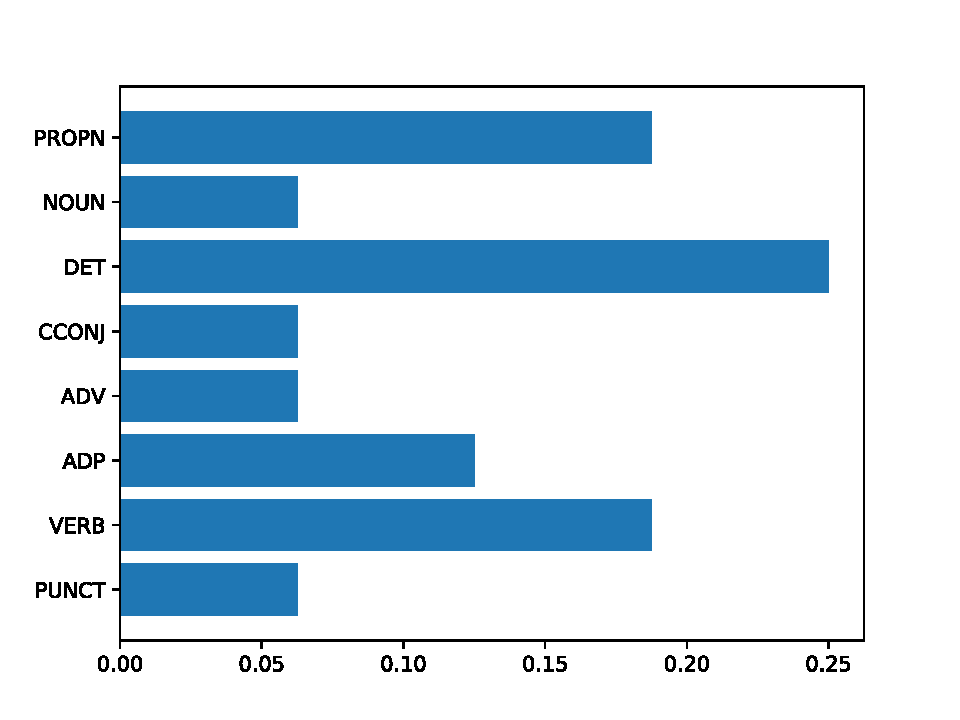
\includegraphics[width=10cm]{Pictures/pos_frequence}}
	\caption{\textit{Output} de invocação da função \textit{generate\_pos\_chart}}
	\label{figure:pos-frequence}
\end{figure}

\subsection{Tabela com informações sobre \textit{Tokens}}

A função \textit{generate\_information} permite obter várias informações sobre os \textit{Tokens} de um documento. Para isso, basta percorrer os \textit{tokens} do \textit{Doc} e aceder aos atributos do mesmo, conforme explicitado previamente. Se o \textit{output} for solicitado no tipo \textit{html}, retorna-se uma tabela nesse formato. Caso contrário, retorna-se uma \textit{PrettyTable} que poderá ser impressa no terminal.

\begin{verbatim}
	>>> import spacy
	>>> from prettytable import PrettyTable
	>>> nlp = spacy.load('en_core_web_lg')
	>>> doc = nlp('We have to go there now!')
	>>> print(generate_information(doc, nlp.vocab, type='text'))
\end{verbatim}

\begin{figure}[!ht]
	\centering
	\setlength{\abovecaptionskip}{-.5cm}
	\makebox[\textwidth][c]{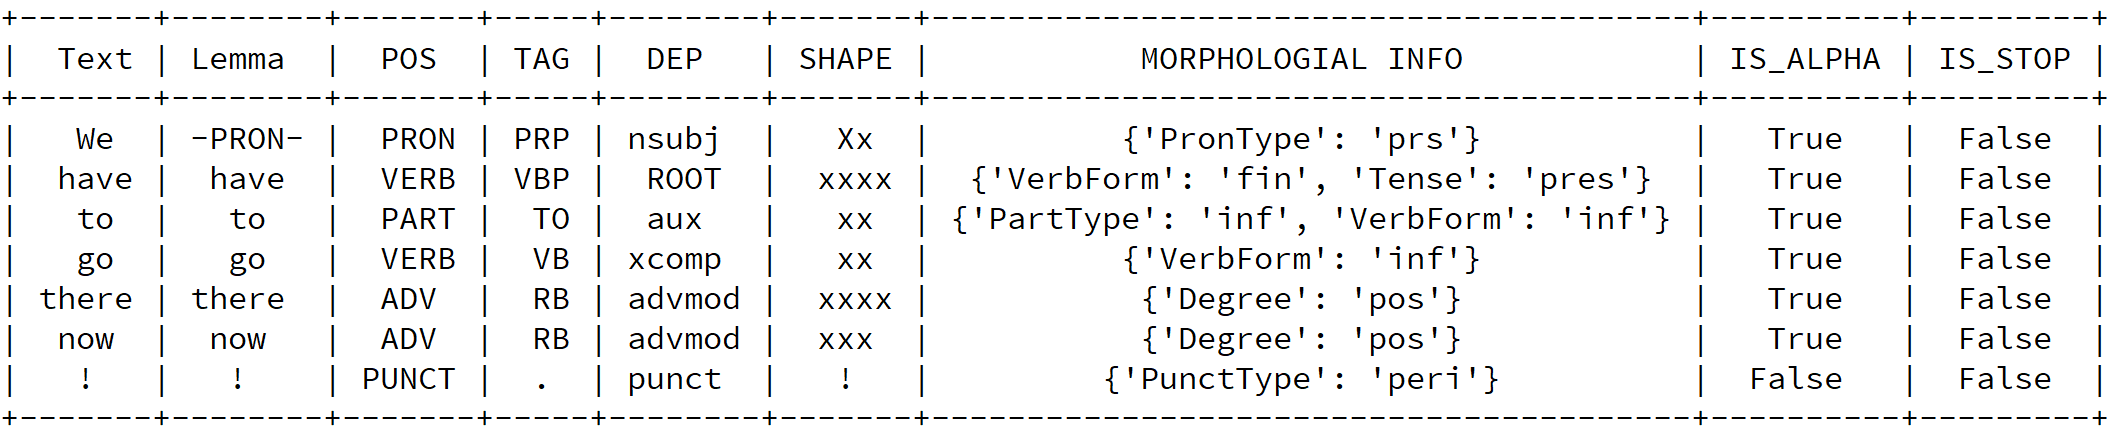
\includegraphics[width=14cm]{Pictures/table_info}}
	\caption{\textit{Output} de invocação da função \textit{generate\_info}}
	\label{figure:table-info}
\end{figure}

\subsection{Resultados}

Os resultados obtidos através da execução via linha de comandos são iguais aos previamente recolhidos para a execução das funções individualmente. No contexto \textit{wed}, apresentam-se nas imagens do anexo {{REF}} exemplos de funcionamento de cada uma das funcionalidades.


% Anexos

\setcounter{section}{0}
\setcounter{subsection}{0}


\newpage

\appendixpage
\renewcommand{\thesubsection}{\Alph{subsection}}

\subsection{\textit{Working Example}: código associado à utilização de spaCy}
\label{anexo:working_example_1}
\begin{minted}[linenos,frame=lines,breaklines]{python}
import os
import re
import pandas as pd
import spacy
from spacy import displacy
from spacy.util import update_exc
from pathlib import Path
from prettytable import PrettyTable
import matplotlib as mpl
mpl.use('Agg')
from matplotlib import pyplot as plt

# Gerar tabelas (auxiliares)
def generate_html_table(headers, data):
    res = '<table class="table table-striped">\n'
    res += '  <thead><tr><th>' + '    </th><th>'.join(headers) + '  </th></tr></thead>\n  <tbody>\n'
    for sublist in data:
        res += '  <tr><td>'
        res += '    </td><td>'.join(sublist)
        res += '  </td></tr>\n'
    res += '  </tbody>\n</table>\n'
    return res

def generate_table(headers, data):
    table = PrettyTable()
    table.field_names = headers
    for row in data:
        table.add_row(row)
    return table


# Part-of-speech tagging
def generate_pos_chart(doc, filename='pos_frequence.svg', type='html'):
    tag_dict = {w.pos : w.pos_ for w in doc}
    pos_freq = []
    pos_tags = []
    for pos_id, freq in doc.count_by(spacy.attrs.POS).items():
        pos_freq.append(freq / len(doc))
        pos_tags.append(tag_dict[pos_id])
    if type=='html':
        return [['POS Tag', 'POS Frequence (%)']] + [list(x) for x in zip(pos_tags,pos_freq)]
    else:
        plt.barh(range(1,len(pos_tags)+1), pos_freq, tick_label=pos_tags)
        plt.savefig(filename)


# Get token's information
def generate_information(doc, vocab, type='html'):
    # python3 -m spacy download pt
    headers = ["Text","Lemma", "POS", "TAG", "DEP", "SHAPE", "MORPHOLOGIAL INFO", "IS_ALPHA", "IS_STOP"]
    data = []
    tokens = []

    for token in doc:

        if (str(token.pos_) != 'SPACE' and str(token.pos_) != 'PUNCT') or token.text not in tokens:

            if token.tag_:
                morph_info = dict(filter(lambda x : x[0]!=74, vocab.morphology.tag_map[token.tag_].items()))
                if not morph_info:
                    morph_info = ''

            else:
                morph_info = ''
            data.append([str(s) for s in (token.text, token.lemma_, token.pos_, token.tag_, token.dep_, token.shape_, morph_info, token.is_alpha, token.is_stop)])
            tokens.append(token.text)

    if type=='html':
        return generate_html_table(headers, data)
    else:
        return generate_table(headers, data)



# Dependencies Graph
def generate_dependencies_graph(doc, type='service', compact = False, background='white', color='black', font='Source Sans Pro'):
    res = []
    if type in ('service', 'html', 'pict'):
        docs = list(doc.sents)
        options = {'compact': compact, 'bg': background, 'color': color, 'font': font}
    if type == 'service':
        displacy.serve(docs, style='dep', options=options)
    elif type == 'html':
        html = displacy.render(docs, style='dep', page=True, options=options)
        html = re.sub(r'.*<body[^>]*>(.*)</body>.*', r'\1', html, flags=re.DOTALL)
        res.append(html)
    elif type == 'pict':
        for doc in docs:
            pict = displacy.render(doc, style='dep', options=options)
            res.append(pict)
    return res



# Visualizing the entity recognizer
def generate_tagged_text(doc, type = 'server', entities = None, colors = None):
    res = ''
    if type in ('server', 'html'):
        options = {}
        if entities:
            options['ents'] = entities
        if colors:
            options['colors'] = colors
        if type=='server':
            displacy.serve(doc, style='ent', options=options)
        else:
            res = displacy.render(doc, style='ent', options=options)
    else:
        res_list = []
        for word in doc:
            if word.ent_type_ and not str(word).isspace():
                res_list.append(str(word) + '{' + word.ent_type_ + '}')
            else:
                res_list.append(str(word))
        res = ' '.join(res_list)
    return res

# Rule-based morphology
def add_tokenizer_exceptions(nlp, tokens, tokenizer=None):
    if not tokenizer:
        tokenizer = nlp.tokenizer
    for token, token_attrs in tokens.items():
        tokenizer.add_special_case(token, token_attrs)
\end{minted}

\newpage

\subsection{\textit{Working Example}: código associado à interação com o utilizador}
\label{anexo:working_example_2}
\begin{minted}[linenos,frame=lines,breaklines]{python}
import sys
import getopt
import json
import spacy
from pos_tagging import *
from flask import Flask, request, url_for, redirect, render_template

# Processar argumentos do comando
def processArgs():
    info_out = ''
    pos_chart_out = ''
    tagged_text_out = ''
    graphs_out = ''
    lang = 'pt'
    inputfile = ''

    error = 'USAGE:\tpython3 app.py [(-i <outputfile> | -p <outputfile> | -t <outputfile> | -g <outputfile>) [-l <language>] <inputfile>]\n\n' + \
            'OPTIONS:\n' + \
            '\t-l\tlanguage - \'pt\' (default) or \'en\'\n' + \
            '\t-i\treturns table with information about tokens to outputfile (or \'shell\')\n' + \
            '\t-p\tgenerates bar chart with POS tag frequence to outputfile\n' + \
            '\t-t\treturns tagged text to outputfile (or \'shell\')\n' + \
            '\t-g\tgenerates dependencies graphs to outputfile.svg\n' +\
            '* if no options are provided, a web server will be initialized, where the input will be inserted and the output presented.'

    # Processar opções/argumentos do comando utilizado
    try: 
        opts, args = getopt.getopt(sys.argv[1:],"i:p:t:g:l:hv", ["info=", "pos-chart=", "tagged-text=", "graphs=", "lang=", "help", "version"])
    except getopt.GetoptError:
        print(error)
        sys.exit(2)
    for opt, arg in opts:
        if opt in ('-h', '--help'):
            print(error)
            sys.exit()
        elif opt in ('-v', '--version'):
            print('Version 1.0')
            sys.exit()
        elif opt in ("-i", "--info"):
            info_out = arg
        elif opt in ("-p", "--pos-chart"):
            pos_chart_out = arg
        elif opt in ("-t", "--tagged-text"):
            tagged_text_out = arg
        elif opt in ("-g", "--graphs"):
            graphs_out = arg
        elif opt in ("-l", "--lang"):
            lang = arg
    if info_out or pos_chart_out or tagged_text_out or graphs_out:
        if len(args) == 1:
            inputfile = args[0]
        else:
            print(error)
            sys.exit(2)
    elif len(args)>0:
        print(error)
        sys.exit(2)

    return info_out, pos_chart_out, tagged_text_out, graphs_out, lang, inputfile

app = Flask(__name__)

@app.route('/', methods=['GET', 'POST'])
def index():
    global lang, nlp, tagged_text, info, graphs, bar_chart
    if request.method == 'POST':
        lang = request.values.get('lang')
        entities = request.form.getlist('entity')
        token_exceptions = json.loads(request.values.get('tokenExceptions'))
        add_tokenizer_exceptions(nlp[lang], token_exceptions)
        doc = nlp[lang](request.values.get('input'))
        tagged_text = generate_tagged_text(doc, type = 'html', entities = entities)
        info = generate_information(doc, nlp[lang].vocab)
        bar_chart = generate_pos_chart(doc, None, type='html')
        graphs = '\n'.join(generate_dependencies_graph(doc, type = 'html'))
        return redirect(url_for('tagged_text_form'))
    return render_template('index.html', lang=lang)


@app.route('/tagged_text_form', methods=['GET', 'POST'])
def tagged_text_form():
    global tagged_text
    if request.method == 'POST':
        return redirect(url_for('index'))
    return render_template('tagged_text_form.html', tagged_text=tagged_text)


@app.route('/info_form', methods=['GET', 'POST'])
def info_form():
    global info, bar_chart
    if request.method == 'POST':
        return redirect(url_for('index'))
    return render_template('info_form.html', table=info, bar_chart=bar_chart)

@app.route('/graphs_form', methods=['GET', 'POST'])
def graphs_form():
    global graphs
    if request.method == 'POST':
        return redirect(url_for('index'))
    return render_template('graphs_form.html', graphs=graphs)


if __name__ == '__main__':
    global tagged_text, info, graphs
    info_out, pos_chart_out, tagged_text_out, graphs_out, lang, inputfile = processArgs()
    if inputfile:
        if lang == 'en':
            nlp = spacy.load('en_core_web_lg')
        else:
            nlp = spacy.load('pt')
        with open(inputfile, 'r') as input:
            doc = nlp(input.read())
        if info_out:
            output = generate_information(doc, nlp.vocab, 'text')
            if info_out == 'shell':
                print(output)
            else:
                with open(info_out, 'w') as fd:
                    fd.write(output)
        if pos_chart_out:
            generate_pos_chart(doc, pos_chart_out, type='pict')
        if tagged_text_out:
            output = generate_tagged_text(doc, 'text', nlp.vocab)
            if tagged_text_out == 'shell':
                print(output)
            else:
                with open(tagged_text_out, 'w') as fd:
                    fd.write(output)
        if graphs_out:
            os.makedirs('./images', exist_ok=True)
            pictures = generate_dependencies_graph(doc, 'pict')
            for i, pict in enumerate(pictures):
                file_name = graphs_out + '_' + str(i) + '.svg'
                output_path = Path('./images/' + file_name)
                with output_path.open('w', encoding='utf-8') as output_file:
                    output_file.write(pict)
    else:
        nlp = {'en': spacy.load('en_core_web_lg'), 'pt': spacy.load('pt') }
        tagged_text = ''
        info = ''
        graphs = ''
        app.run()
\end{minted}

\newpage

\subsection{Exemplo de aplicação: Treino do \textit{dependency parser} (e serialização)}
\label{anexo:treino}

\begin{minted}[linenos,frame=lines,breaklines]{python}
#!/usr/bin/env python

# https://spacy.io/usage/examples#parser

from __future__ import unicode_literals, print_function

import plac
import random
from pathlib import Path
import spacy
from spacy.util import minibatch, compounding


# training data
TRAIN_DATA = [
    ("They trade mortgage-backed securities.", {
        'heads': [1, 1, 4, 4, 5, 1, 1],
        'deps': ['nsubj', 'ROOT', 'compound', 'punct', 'nmod', 'dobj', 'punct']
    }),
    ("I like London and Berlin.", {
        'heads': [1, 1, 1, 2, 2, 1],
        'deps': ['nsubj', 'ROOT', 'dobj', 'cc', 'conj', 'punct']
    })
]

@plac.annotations(
    model=("Model name. Defaults to blank 'en' model.", "option", "m", str),
    output_dir=("Optional output directory", "option", "o", Path),
    n_iter=("Number of training iterations", "option", "n", int))

def main(model=None, output_dir=None, n_iter=10):
    """Load the model, set up the pipeline and train the parser."""
    if model is not None:
        nlp = spacy.load(model)  # load existing spaCy model
        print("Loaded model '%s'" % model)
    else:
        nlp = spacy.blank('en')  # create blank Language class
        print("Created blank 'en' model")

    # add the parser to the pipeline if it doesn't exist
    # nlp.create_pipe works for built-ins that are registered with spaCy
    if 'parser' not in nlp.pipe_names:
        parser = nlp.create_pipe('parser')
        nlp.add_pipe(parser, first=True)
    # otherwise, get it, so we can add labels to it
    else:
        parser = nlp.get_pipe('parser')

    # add labels to the parser
    for _, annotations in TRAIN_DATA:
        for dep in annotations.get('deps', []):
            parser.add_label(dep)

    # get names of other pipes to disable them during training
    other_pipes = [pipe for pipe in nlp.pipe_names if pipe != 'parser']
    with nlp.disable_pipes(*other_pipes):  # only train parser
        optimizer = nlp.begin_training()
        for itn in range(n_iter):
            random.shuffle(TRAIN_DATA)
            losses = {}
            # batch up the examples using spaCy's minibatch
            batches = minibatch(TRAIN_DATA, size=compounding(4., 32., 1.001))
            for batch in batches:
                texts, annotations = zip(*batch)
                nlp.update(texts, annotations, sgd=optimizer, losses=losses)
            print('Losses', losses)

    # test the trained model
    test_text = "I like securities."
    doc = nlp(test_text)
    print('Dependencies', [(t.text, t.dep_, t.head.text) for t in doc])

    # save model to output directory
    if output_dir is not None:
        output_dir = Path(output_dir)
        if not output_dir.exists():
            output_dir.mkdir()
        nlp.to_disk(output_dir)
        print("Saved model to", output_dir)

        # test the saved model
        print("Loading from", output_dir)
        nlp2 = spacy.load(output_dir)
        doc = nlp2(test_text)
        print('Dependencies', [(t.text, t.dep_, t.head.text) for t in doc])


if __name__ == '__main__':
    plac.call(main)

    # expected result:
    # [
    #   ('I', 'nsubj', 'like'),
    #   ('like', 'ROOT', 'like'),
    #   ('securities', 'dobj', 'like'),
    #   ('.', 'punct', 'like')
    # ]
\end{minted}

\newpage

\subsection{\textit{Working Example}: interface \textit{web}}
\label{anexo:working_example_web}

\begin{figure}[!ht]
	\centering
	\setlength{\abovecaptionskip}{-.4cm}
	\makebox[\textwidth][c]{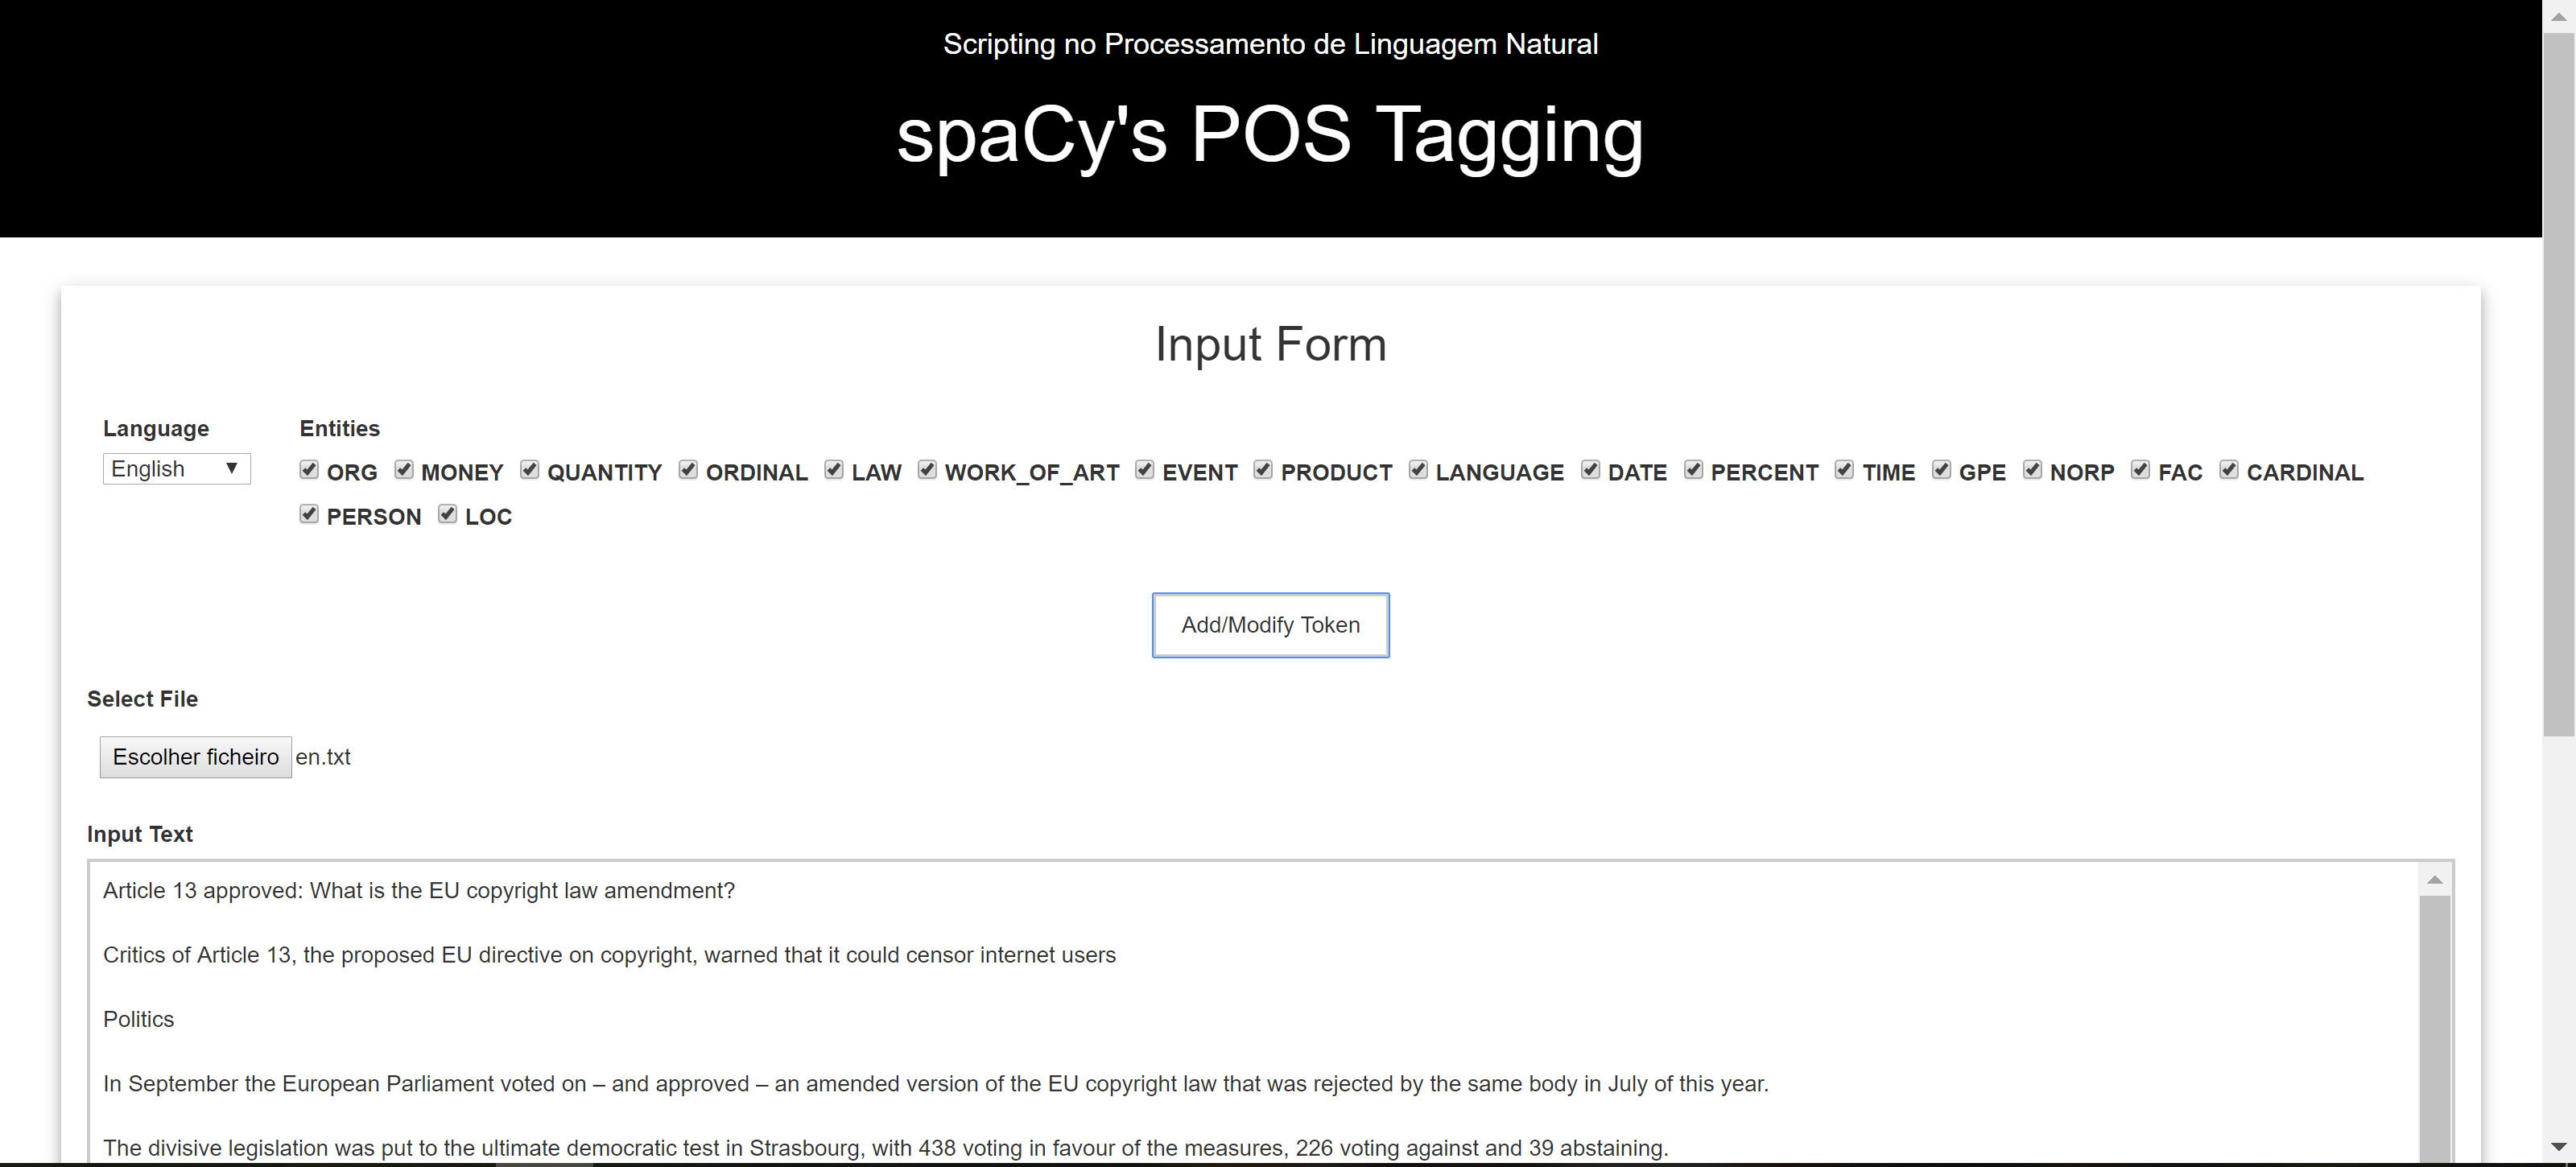
\includegraphics[width=16cm]{Pictures/web_index}}
	\caption{Página inicial onde se indica a linguagem, as entidades a etiquetar e o \textit{input}}
\end{figure}

\begin{figure}[!ht]
	\centering
	\setlength{\abovecaptionskip}{-.4cm}
	\makebox[\textwidth][c]{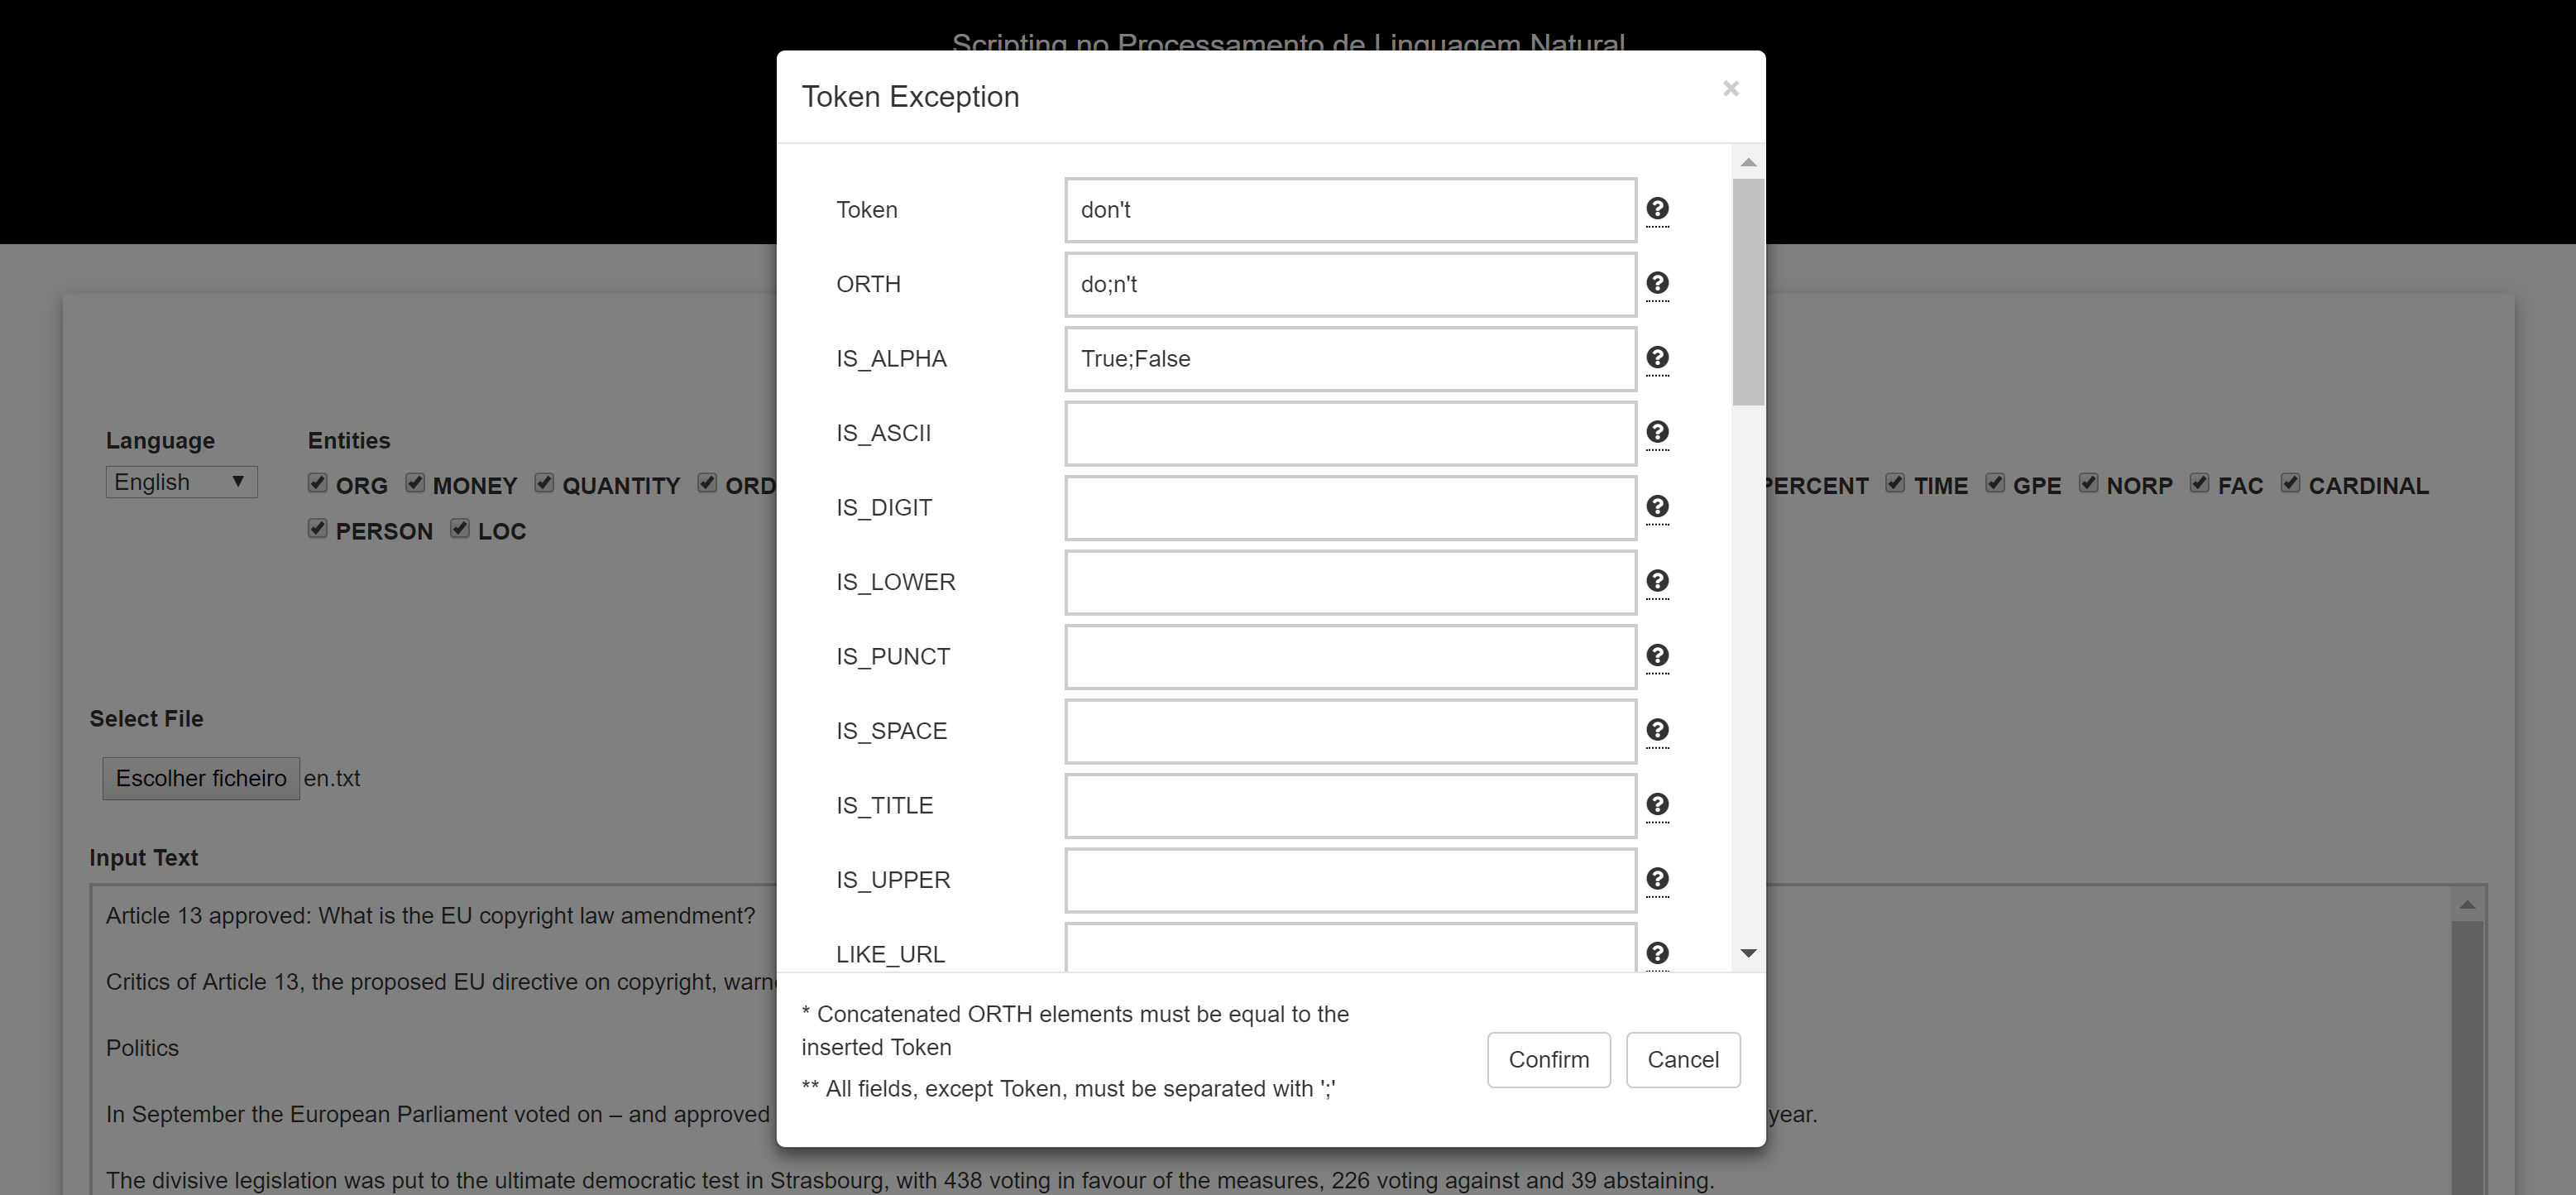
\includegraphics[width=16cm]{Pictures/web_token_exception}}
	\caption{Modal da página inicial, onde se especifica um caso especial de \textit{Token}}
\end{figure}

\begin{figure}[!ht]
	\centering
	\setlength{\abovecaptionskip}{-.4cm}
	\makebox[\textwidth][c]{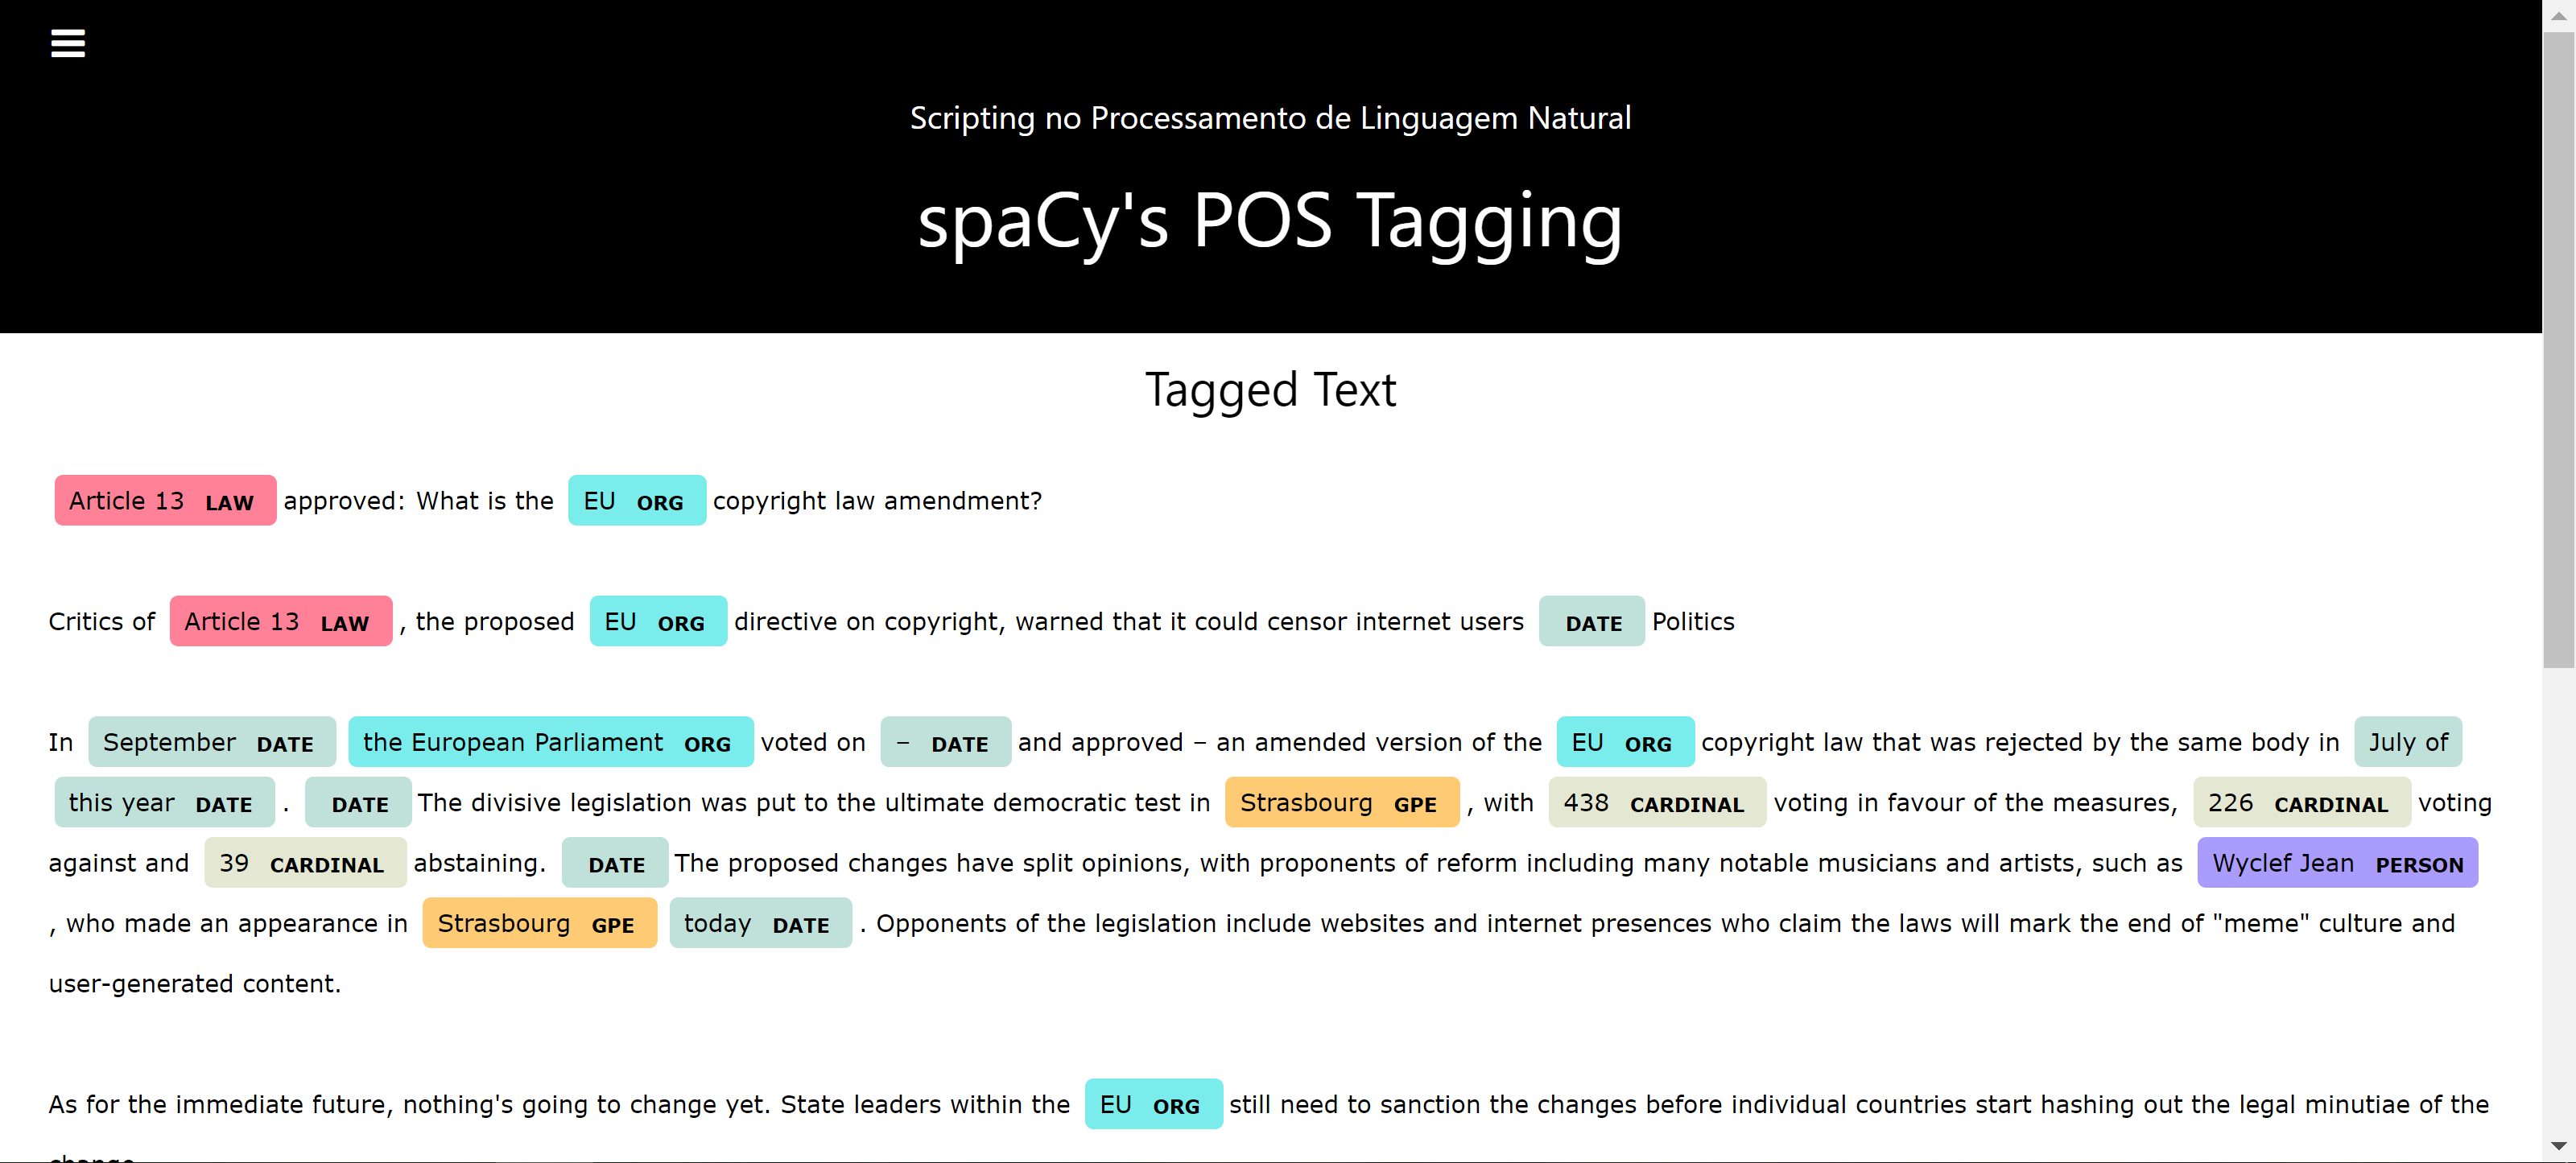
\includegraphics[width=16cm]{Pictures/web_ent_tagged_text}}
	\caption{Página que apresenta o texto de \textit{input} com as entidades etiquetadas}
\end{figure}

\begin{figure}[!ht]
	\centering
	\setlength{\abovecaptionskip}{-.4cm}
	\makebox[\textwidth][c]{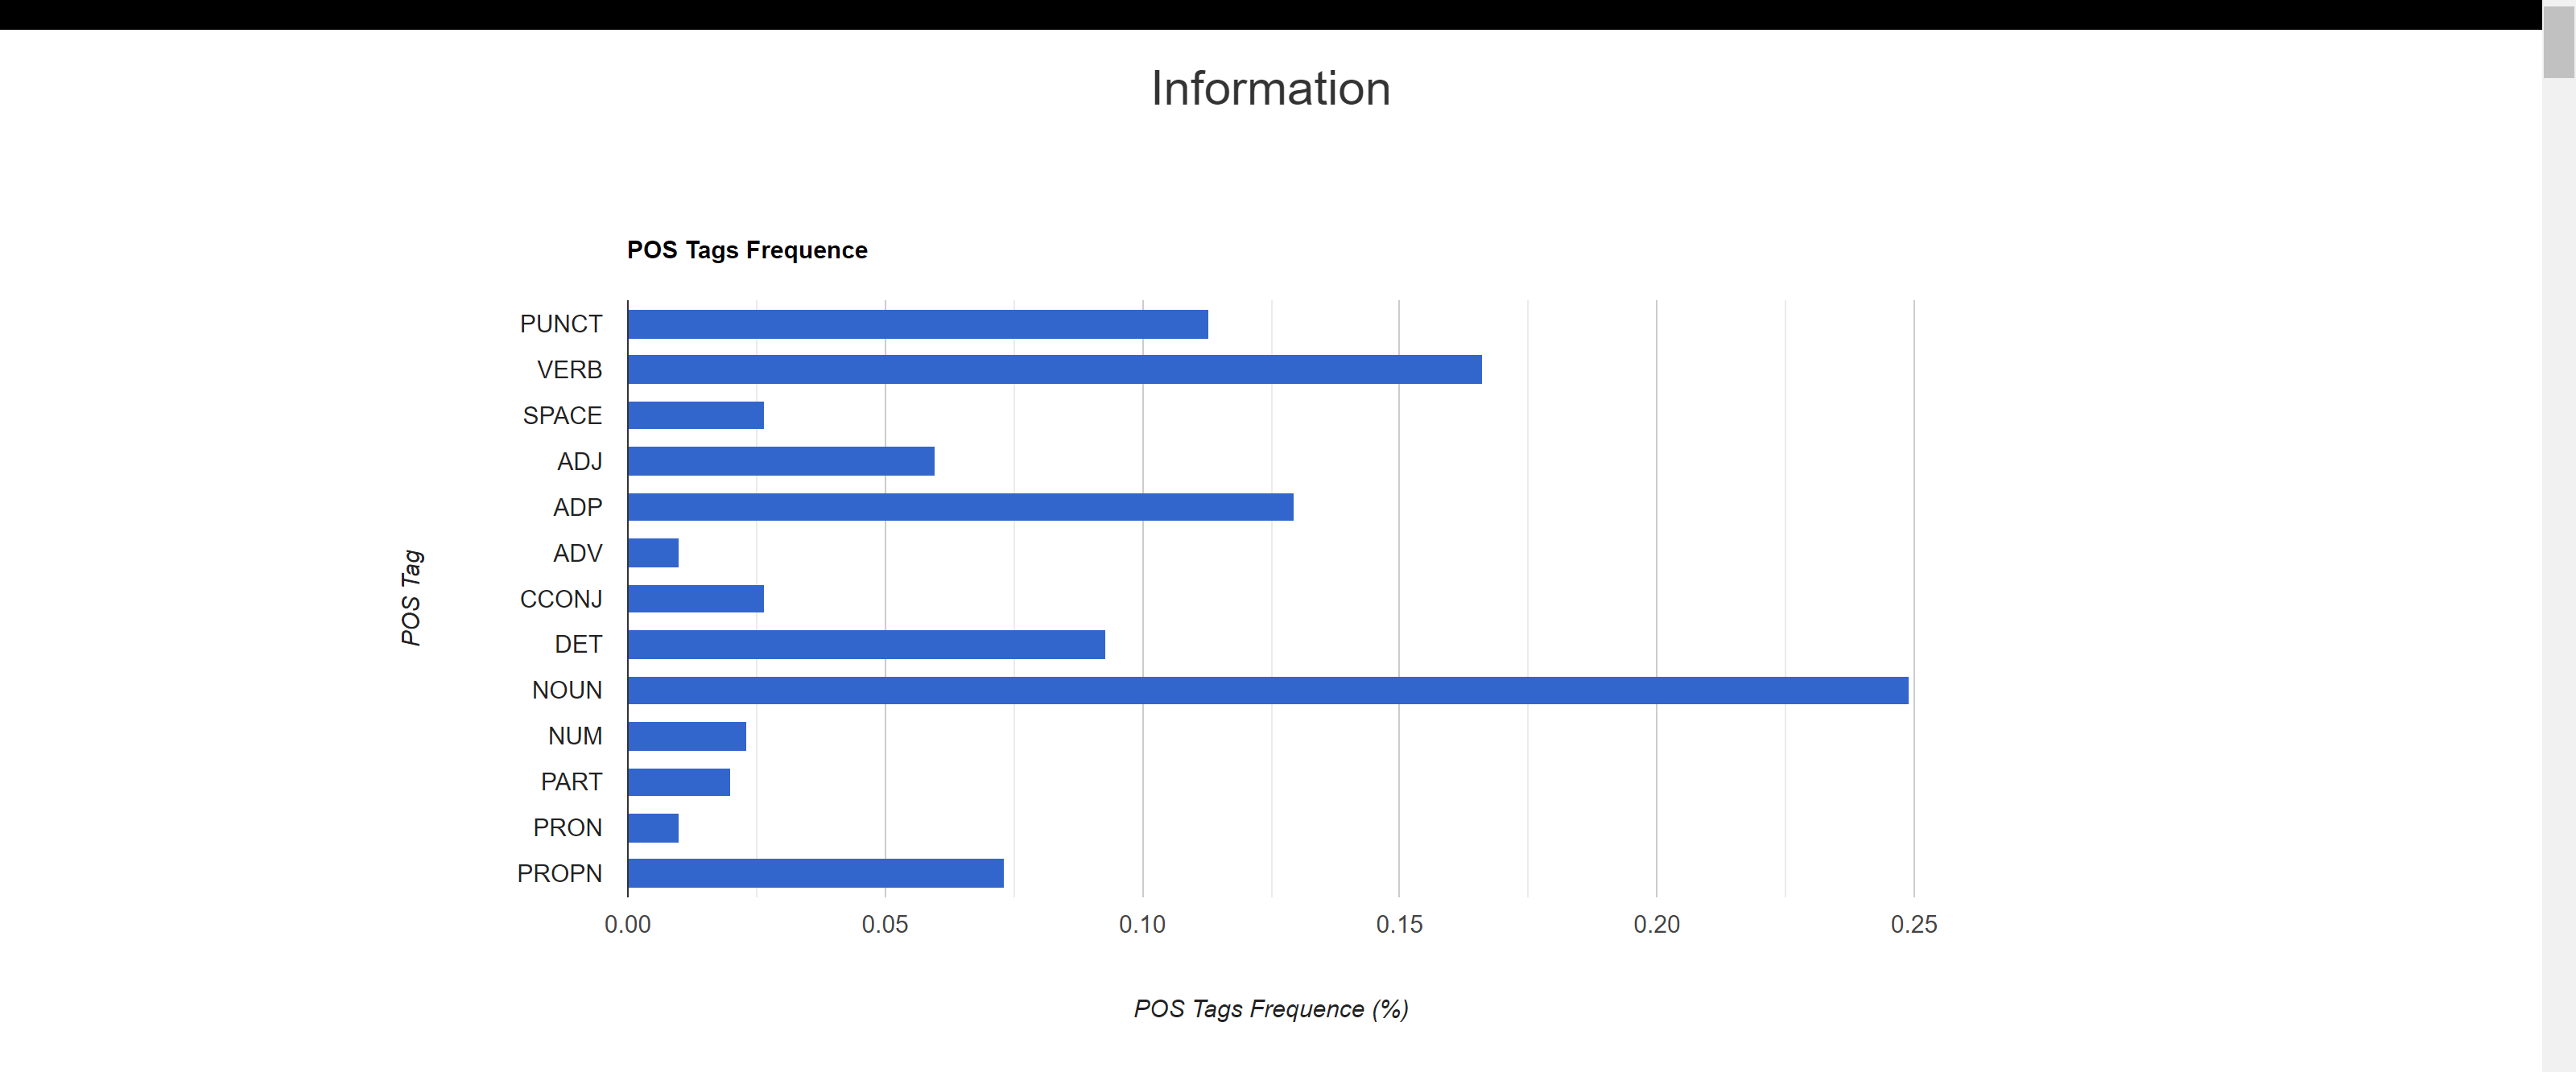
\includegraphics[width=16cm]{Pictures/web_bar_chart}}
	\caption{Excerto de página que apresenta a taxa de ocorrência de cada POS}
\end{figure}

\begin{figure}[!ht]
	\centering
	\setlength{\abovecaptionskip}{-.4cm}
	\makebox[\textwidth][c]{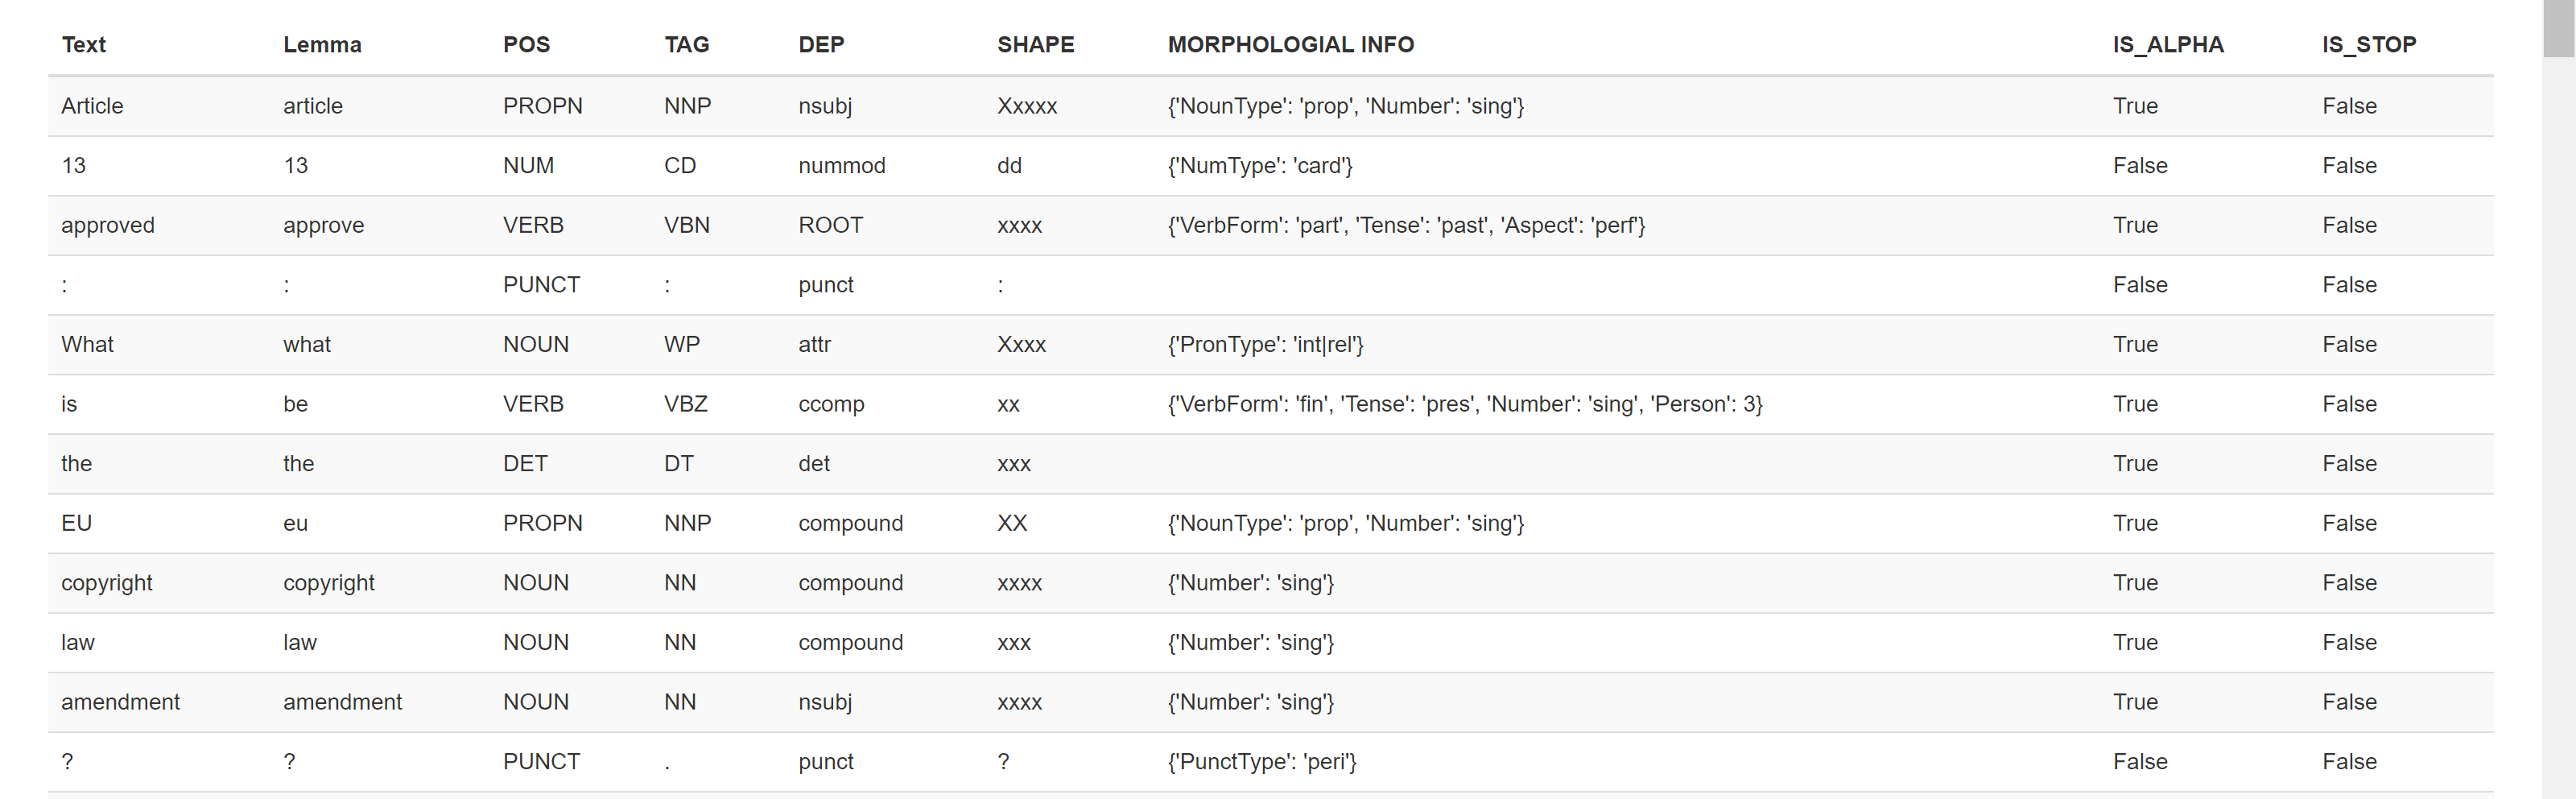
\includegraphics[width=16cm]{Pictures/web_info}}
	\caption{Excerto de página que apresenta informações sobre cada token do texto inicial}
\end{figure}

\begin{figure}[!ht]
	\centering
	\setlength{\abovecaptionskip}{-.4cm}
	\makebox[\textwidth][c]{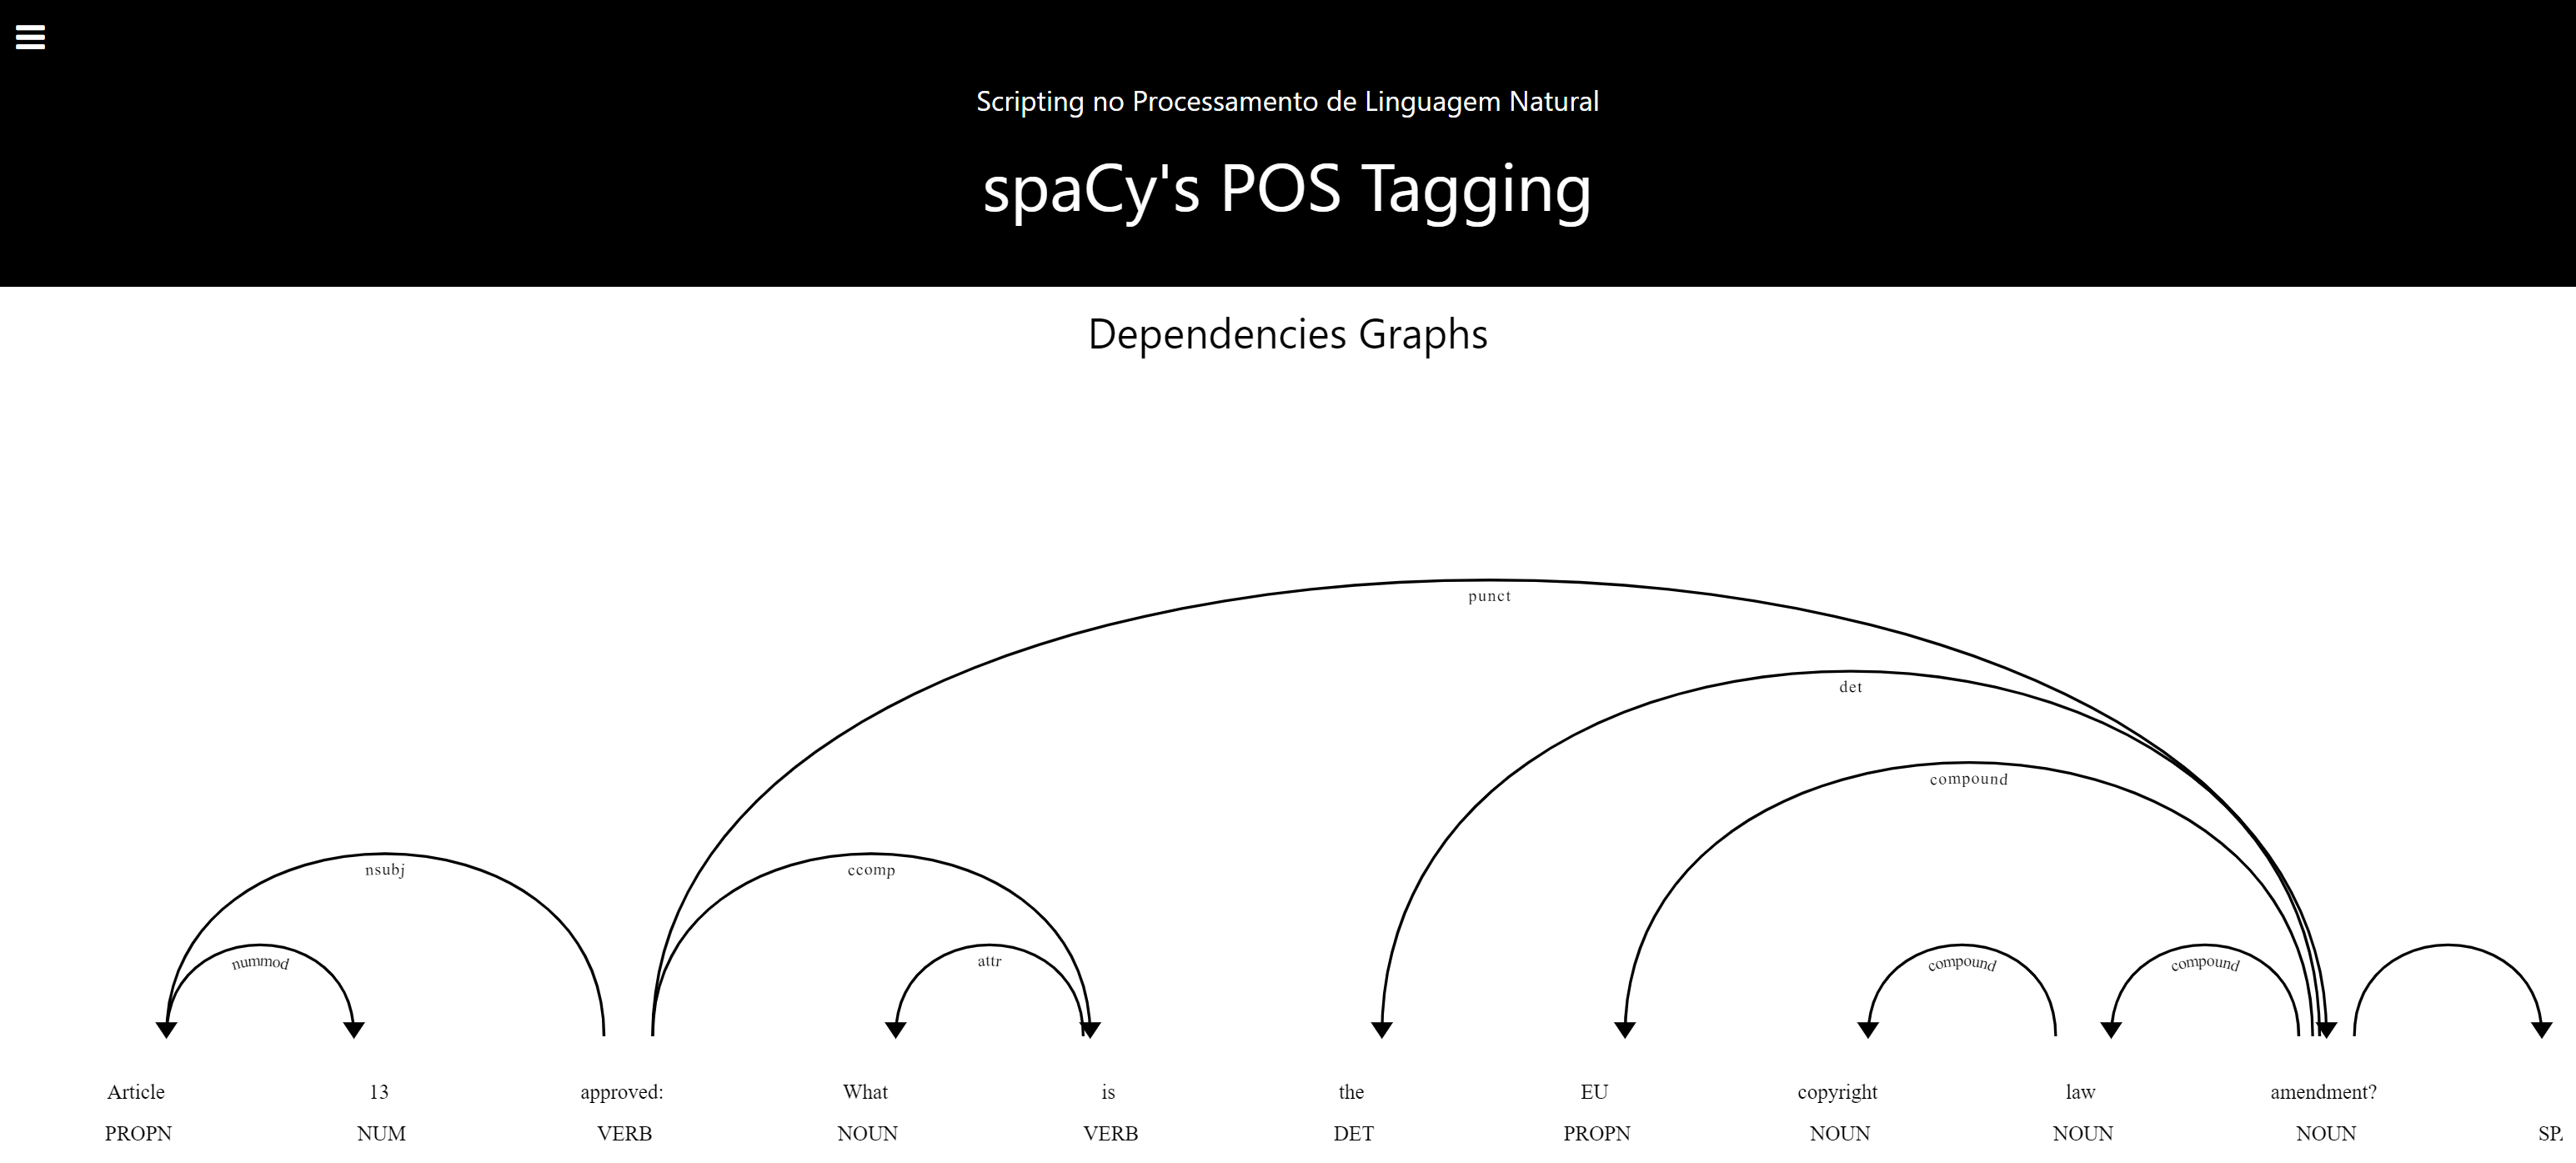
\includegraphics[width=16cm]{Pictures/web_dep_graph}}
	\caption{Página que apresenta grafos de dependências de cada frase do texto inicial}
\end{figure}


\clearpage

\begin{thebibliography}{99}
	
	\bibitem{linkname}
	Autor,
	``Título'',
	\textit{website name},
	\url{website link}.
	
\end{thebibliography}

\end{document}